%% LaTeX - Jesus Villota's Paper Template %% 

\documentclass[12pt,a4paper]{article}
\usepackage{/Users/jesusvillotamiranda/Documents/LaTeX/JVM_Macros}

%----------------------------------------------------
\title{\textsc{
\Large 
%Highly-leveraged Dollar-neutral Copula-based  
Pairs-Trading %with 
a Sparse Synthetic Control 
}
}

\author[1]{
{ 
{\large Jesus Villota Miranda}$^{\dagger}$\footnote{
\scriptsize{
%I am deeply grateful to [...].
%Finally, 
I gratefully acknowledge financial support from the Santander Research Chair at CEMFI.
}
}}

\bx 
{\small
$\big{<}$
\noindent $^{\dagger}$CEMFI, Calle Casado del Alisal, 5, 28014 Madrid, Spain 
$\big{>}$

$\big{<}$
Email: \href{mailto:jesus.villota@cemfi.edu.es}{\texttt{jesus.villota@cemfi.edu.es}}
$\big{>}$

\textbf{This version: \mydate\today}
}
}
\date{}
%----------------------------------------------------

%%%%%%%%%%%%%%%%%%%%%%%%%%%%%%%%%%%%%%%%%%%%%%%%%%%%%
%%%%%%%%%%%%%%%%%%%%%%%%%%%%%%%%%%%%%%%%%%%%%%%%%%%%%
\begin{document}
\maketitle
\thispagestyle{empty}
%----------------------------------------------------
\begin{abstract}
%{\footnotesize 
This paper defines a novel approach to pairs trading by borrowing the concept of synthetic control from the treatment literature. In this paper we select a stock (termed \qquote{target}) and construct its replica as a sparse linear combination of other assets (termed \qquote{synthetic}). Then, we perform pairs trading on the target vs. synthetic assets; for this purpose, we (nonlinearly) model their joint dependence via a Student-$t$ copula and then construct mispricing indices from the implied conditional densities. Finally, we feed the dynamics of our miscpricing indices to a reinforcement learning agent. Our findings show that our RL agent succesfully implement statistical arbitrage based on our mispricing signals with a high net profitability out of sample. 


%Financial markets frequently exhibit transient price divergences between economically linked assets, yet traditional pairs trading strategies struggle to adapt to structural breaks and complex dependencies, limiting their robustness in dynamic regimes.
%%
%This paper addresses these challenges by developing a novel framework that integrates sparse synthetic control with copula-based dependence modeling to enhance adaptability and risk management.
%%
%Economically, our approach responds to the need for strategies that systematically identify latent linkages while mitigating overfitting in high-dimensional asset pools.
%%
%The sparse synthetic control methodology constructs a parsimonious synthetic asset via an $\ell_1$-regularized least squares optimization, which automatically selects a sparse subset of assets from a broad donor pool while maintaining interpretability and computational efficiency.
%%
%By embedding this within a copula-based dependence framework, we capture non-linear and tail dependencies between target and synthetic assets.
%%
%Trading signals, grounded in the relative mispricing between these assets, employ a cumulative index that resets after position closures to isolate episodic opportunities, with disciplined entry rules requiring concurrent misalignment signals to filter noise.
%%
%Empirical analysis demonstrates the superior performance of our approach across diverse market conditions. 

\bx 
\noindent\textbf{JEL Codes:} C14, C32, C58, C61, G12, G14

\mx 
\noindent\textbf{Keywords:} Pairs Trading, Sparse, Synthetic Control, High leverage, Dollar neutral, Copula, 
%\par }
\end{abstract}
%----------------------------------------------------

\newpage
\setcounter{page}{1}

%%%%%%%%%%%%% INTRODUCTION %%%%%%%%%%%%%%%%%%
\section{Introduction}

%----------------------------------------------------
%%%%%%%%%%%%%%%%%%%%%%%%%%%%%%%%%%%%%%%%%%%%%%%%%%%%%
% Definitive
%%%%%%%%%%%%%%%%%%%%%%%%%%%%%%%%%%%%%%%%%%%%%%%%%%%%%

%====================[Pairs Trading]=========================

% ------[ Definition: What is it? ]-------

Pairs trading is widely recognized as a cornerstone of statistical arbitrage, offering a market-neutral investment approach that exploits temporary divergences in the prices of historically correlated or economically linked assets.
%
% ------[ Explanation: What does it involve? ]-------
%
By simultaneously taking a long position in the relatively undervalued asset and a short position in the relatively overvalued one, pairs traders aim to profit from the eventual convergence of these prices. This strategy has garnered enduring prominence among quantitative researchers and practitioners, attributing its appeal to both conceptual simplicity--focusing on the relative mispricing of two assets--and the potential for stable returns independent of broader market movements.

% ------[ Challenges / Limitations ]-------

While pairs trading is conceptually straightforward, its effective implementation faces notable complexities in practice. Traditional approaches often rely on simple distance measures or cointegration-based criteria to identify pairs and establish entry and exit rules. However, these methods can be hampered by strict parametric assumptions, sensitivity to transient noise, and an inability to adapt to evolving market conditions. Structural breaks, non-linear dependencies, and time-varying correlation patterns often violate the assumptions of classical linear models, increasing the risk of identifying spurious relationships and making it difficult to achieve stable performance over diverse market regimes.

To address these challenges, recent research has explored more flexible frameworks that combine advanced econometric tools with statistical learning. In particular, incorporating synthetic control methodologies and copula-based dependence modeling aims to better capture the dynamic interactions between assets. By abandoning the sole reliance on fixed, potentially fragile pair relationships, such approaches promise to more robustly uncover the underlying economic or statistical linkages that drive temporary mispricings, thus laying the groundwork for improved performance and risk control in pairs trading strategies.

%====================[This paper]=========================

Building on the challenges and limitations outlined above, this paper proposes a novel pairs trading framework that integrates sparse synthetic control methods with copula-based dependence modeling. 
%
% ------[ Research Question ]-------
%
The primary research question we aim to answer is: \qquote{Can the integration of sparse synthetic control and copula-based dependence modeling improve the performance of pairs trading strategies?}
%
% ------[ How we address this question ]-------
%
To address this question, we design a methodology that overcomes several shortcomings of traditional pairs trading. 

First, rather than relying on a fixed or pre-specified partner asset, we construct a \emph{synthetic asset} through a sparse linear combination of assets from a larger donor pool. This allows the framework to discover the most influential contributors to the target asset's behavior, effectively automating pair selection. By enforcing sparsity in the weight vector, we reduce computational complexity and enhance interpretability, while mitigating overfitting risks in thinner markets.

Second, we incorporate copula-based dependence modeling to capture potentially complex, non-linear relationships and tail dependencies that can arise in financial returns. Unlike correlation- or cointegration-based strategies, which often impose strict distributional assumptions, copulas decouple the marginal distributions from the joint dependence structure, thereby offering a more nuanced view of how assets co-move. This feature is especially important in periods of market stress, when returns frequently exhibit heightened correlations and non-linearities.

Finally, we adapt and extend the Mispricing Index (MI) strategy of \cite{Xie2016} by introducing a Cumulative Mispricing Index (CMI) that resets upon trade closure, ensuring that stale signals do not accumulate across different trading episodes. As in \cite{Rad2016}, we adopt an \qquote{AND-OR} logic for opening and closing positions, requiring persistent mispricing signals from both the target and synthetic assets to initiate a trade and closing positions promptly when either market correction or stop-loss conditions are met.

%====================[Structure]=========================

The remainder of this paper proceeds as follows. 
%
In Section 1 %\cref{sec:literature_review} 
we begin by reviewing the relevant literature on pairs trading, synthetic control methods, and copula-based dependence modeling. 
%
In Section 2 %\cref{sec:methodology} 
we present our methodological framework, detailing how sparse synthetic control and copula families are jointly employed to construct a robust trading signal, and introduce the mispricing index (MI) strategy adapted to incorporate copula-driven signals. 
%
Subsequently, in Section 3 %\cref{sec:empirics}
we conduct an empirical evaluation using real-world market data, illustrating the performance and practical implications of our approach. 
%
We conclude in Section 4 %\cref{sec:conclusion} 
by summarizing key insights, discussing limitations, and outlining prospective directions for future research.

%----------------------------------------------------

\subsection{Literature Review}

%%----------------------------------------------------
%%Your task will be to help me generate a literature review for the paper. I will provide you a JSON schema with information extracted from each of the references I wish to review. In each schema, there is a "citation" field, which you will use to cite each of the papers when you generate the literature review. You will produce a literature revision following the guidelines of this document, such guidelines will be written as latex comments (starting with a %). The literature revision will be structured in paragraphs, and each paragraph corresponds to a thematic revision (classics, cointegration-based, empirical investigation, didactic sources, copula-based, other approaches, index-tracking). Use the JSON schema with the information of each paper to produce an informed revision, note that the field "citation" provides the bibtex reference that will allow you to map each reference to the ones provided here. Produce your literature revision in tex code. 


%----------------------------------------------------
% Here, I just want to refer to some of the pioneering work in pairs trading. Your revision here should be focused on referring to this papers as foundational or as key references in the development of reserach in pairs trading.
\qquote{Pairs Trading Classics}
\begin{itemize}
  \item \cite{Gatev2006}
  \item \cite{Elliott2005}
\end{itemize}

%----------------------------------------------------
\qquote{Cointegration-based} % here just mention that traditionally, a propular approach has been to approach pairs trading from a cointegration approach. 
\begin{itemize}
  \item \cite{vidyamurthy2004pairs} % you should mention that this book is a foundational reference in the application of cointegration analysis to pairs trading. and then, review the following papers in order (note that it is chronological). give a one liner for each paper (note that we don't care per se about the results of these papers, we just want to mention them as evidence that there is a strand of literature devoted to exploring cointegration-based pairs trading) 
  \item \cite{Caldeira2013}
  \item \cite{Huck2014}
  \item \cite{Cartea2015}
  \item \cite{Lintilhac2016}
\end{itemize}

%----------------------------------------------------
\qquote{Empirical investigations of pairs trading} % these are papers that study the profitability of the pairs trading strategy. simply say that these papers have investigated the profitability of pairs trading and give a one or two liner about the specifics of each paper.
\begin{itemize}
  \item \cite{Chen2019}
  \item \cite{Do2010}
  \item \cite{Bowen2014}
  \item \cite{Krauss2016}
  \item \cite{Rad2016} % this paper investigates different pairs trading frameworks: distance-based, cointegration-based and copula-based)
\end{itemize}

%----------------------------------------------------
\qquote{Didactic sources} % these are some didactic references for the interested reader. briefly review them following these guidelines:
\begin{itemize}
  \item \cite{hudsonthames2024} % this books contains a comprehensive guide to pairs trading. it reviews from a practical perspective all the different ways in which pairs trading has been approached in the literature
  \item \cite{alexander2008market} % this book contains a great introduction to the topics of cointegration along with a practical presentation of it applied to pairs trading (chapter II.5), and also gives a great introduction to the use of copulas for financial applications (in chapter II.6), that's it.
\end{itemize}

%----------------------------------------------------
\qquote{Copula-based pairs trading} % here i want to devote a paragraph or two to reviewing with more detail the copula-based pairs trading approaches. we want to review each reference in a one or two-liner, trying to connect the dots. 
\begin{itemize}
  \item \cite{Min2010}
  \item \cite{stander2013trading}
  \item \cite{Liew2013}, \cite{Xie2016}
  \item \cite{lau2016multi}
  \item \cite{Krauss2017}
  \item \cite{zhi2017dynamic}
  \item \cite{Chu2018}
  \item \cite{SabinodaSilva2023}
  \item \cite{Wang2023}
  \item \cite{He2024}
  \item \cite{Tadi2025}
\end{itemize}

%----------------------------------------------------
\qquote{Pairs Trading: other approaches} % here i just want to mention that alternative approaches have been proposed to the pairs trading framework. review briefly the general idea of each paper in a one-liner. the result should be a paragraph where i explain alterantive approaches to pairs trading.
\begin{itemize}
  \item \cite{do2006new}
  \item \cite{Zeng2014} 
  \item \cite{Sarmento2020}, 
  \item \cite{Johansson2024}
  \item \cite{Han2023}
  \item \cite{qureshi2024pairs}
  \item \cite{Roychoudhury2023}
  \item \cite{Rotondi2025}
\end{itemize}

%----------------------------------------------------
\qquote{Synthetic Controls / Index-tracking} % the intention of reviewing these references is to talk about index tracking as somehow inspiring our synthetic control methodology, by which we are using a basket of assets to replicate the price behavior of a target asset (which in these references is the index). review these references shortly, the main goal of this paragraph will be to provide some theoretical background or underpinning for our synthetic control methodology, but we don't care per se about the results of these papers (we simply want to mention them and provide a one-liner with some general statment about each)
\begin{itemize}
  \item \cite{Alexander1999} 
  \item \cite{Alexander2002}
  \item \cite{Alexander2005a}
  \item \cite{Alexander2005b}  
  \item \cite{Shu2020}
  \item \cite{Bradrania2021}
\end{itemize}
%%----------------------------------------------------

%----------------------------------------------------
\subsection{Literature Review} \label{sec:lierature_review}

%==============[	  Classics  ]==============
%Pairs trading has emerged as a cornerstone of statistical arbitrage strategies, with a rich history in both academic research and practical applications. 
The foundational work of \cite{Gatev2006} provided the first comprehensive academic study of pairs trading, documenting significant excess returns of up to 11\% annually for self-financing portfolios over a 40-year period from 1962 to 2002. This seminal paper was complemented by the theoretical framework developed in \cite{Elliott2005}, which introduced a mean-reverting Gaussian Markov chain model for spread dynamics and established analytical methods for parameter estimation using the EM algorithm.

%==============[	  Empirical investigations  ]==============
Empirical investigations have thoroughly examined the profitability of pairs trading across different markets and time periods. For instance, \cite{Chen2019} reported large abnormal returns driven by short-term reversals and pairs momentum effects, while \cite{Do2010} showed that simple pairs trading remains viable in turbulent periods despite a general profitability decline in later years. In a UK-centric study, \cite{Bowen2014} recorded moderate annual returns once risk and liquidity were accounted for. Large-scale assessments in \cite{Krauss2016} and \cite{Rad2016} confirmed that distance, cointegration, and copula-based strategies can yield significant alpha but exhibit important differences regarding convergence speed and trading frequencies.

%==============[	  Cointegration  ]==============
A popular way to identify and exploit persistent relationships in pairs trading has involved cointegration analysis. \cite{vidyamurthy2004pairs} stands out as a seminal reference, detailing how cointegration can be applied to detect mean-reverting spreads in equity markets. 
Subsequent research has explored various aspects of this approach: \cite{Caldeira2013} demonstrated the effectiveness of cointegration-based selection methods in the Brazilian market, while \cite{Huck2014} provided evidence that cointegration-based strategies outperform distance-based methods. \cite{Cartea2015} extended the framework by incorporating optimal dynamic investment strategies, and \cite{Lintilhac2016} applied these techniques to cryptocurrency markets.

%==============[	  Copulas  ]==============
A growing strand of research leverages copulas to model more general dependencies beyond linear correlation.
\cite{Min2010} introduced Bayesian inference for multivariate copulas using pair-copula constructions, while \cite{stander2013trading} offer a copula-based approach for detecting relative mispricing. 
Extensions in \cite{Liew2013} and \cite{Xie2016} underscore that copulas outperform distance-of-prices rules in capturing tail dependencies.
Multi-dimensional variants have been proposed (e.g., \cite{lau2016multi}) to incorporate three or more assets into a single framework. Further refinements, like those introduced in \cite{Krauss2017} and \cite{zhi2017dynamic}, combine t-copulas or dynamic copula-GARCH models with individualized thresholds for improved risk-adjusted returns. In the high-frequency domain, \cite{Chu2018} showed that copula-based mispricing indices can be coupled with deep learning for profitability enhancements. Recent efforts also explore mixed copulas (\cite{SabinodaSilva2023}), ARMA-GARCH approaches (\cite{Wang2023}), and copulas specialized for cointegrated assets (\cite{He2024}), culminating in improved alpha extraction. Finally, \cite{Tadi2025} proposes reference-asset-based copula trading specifically for cryptocurrencies. 
%

%==============[	  Didactic resources  ]==============
Practical guidance and pedagogical discussions on pairs trading can be found in \cite{hudsonthames2024}, which provides a broad compendium of methods, from classical cointegration to machine learning-based selection. On a methodological note, \cite{alexander2008market} offers valuable introductions to both cointegration analysis and copula applications in financial markets, particularly in chapters II.5 and II.6.


%==============[	  Alternative approaches  ]==============
Beyond cointegration or copula methodologies, several innovative techniques have surfaced. 
%New approaches to modeling and parameter estimation for pairs trading appear in \cite{do2006new} and \cite{Zeng2014}, with the latter introducing threshold-based mean-reversion strategies. 
\cite{do2006new} developed a stochastic residual spread model, while \cite{Zeng2014} focused on optimal threshold determination. 
In more recent research, \cite{Sarmento2020} incorporates machine learning (OPTICS clustering) to constrain search space, while \cite{Johansson2024} leverages convex-concave optimization for multi-asset statistical arbitrage. Reinforcement learning is featured in \cite{Han2023} for automated pair selection, and \cite{qureshi2024pairs} employs a graphical matching approach to reduce overlap among chosen pairs. Further, \cite{Roychoudhury2023} couples clustering with deep RL for equity indices, whereas \cite{Rotondi2025} applies a partial correlation-based distance to cluster promising trading candidates.
%Alternative approaches to traditional pairs trading have been proposed. \cite{do2006new} developed a stochastic residual spread model, while \cite{Zeng2014} focused on optimal threshold determination. Machine learning applications have gained prominence, with \cite{Sarmento2020} utilizing LSTM networks, \cite{Han2023} employing unsupervised learning for pair selection, and \cite{Roychoudhury2023} combining clustering with deep reinforcement learning. Novel optimization approaches include the convex-concave framework of \cite{Johansson2024}, the graphical matching approach of \cite{qureshi2024pairs}, and the clustering-based methodology of \cite{Rotondi2025}.
%

%==============[	  Synthetic Controls / Index-Tracking  ]==============
The method of replicating a target asset's returns by constructing a portfolio of contributor assets is reminiscent of index-tracking procedures. Classic treatments connecting cointegration analysis and hedging tasks (e.g., \cite{Alexander1999} and \cite{Alexander2002}) lay theoretical groundwork for such an approach. Subsequent refinements in \cite{Alexander2005a} and \cite{Alexander2005b} investigate how cointegration outperforms traditional techniques in crafting robust index trackers and exploiting time-varying market regimes. Complementary research (e.g., \cite{Shu2020}) shows that sparse solutions across a large universe can reduce transaction costs, an idea further corroborated in \cite{Bradrania2021}, where machine learning identifies dynamic selection methods for index constituents. These frameworks illustrate how synthetic control concepts provide a flexible foundation for building market-neutral positions or tracking assets with fewer assumptions.
%Our synthetic control methodology draws inspiration from the index tracking literature. \cite{Alexander1999} pioneered the application of cointegration to tracking problems, while \cite{Alexander2002} and \cite{Alexander2005a} developed enhanced indexing strategies. \cite{Alexander2005b} explored market regime effects, and recent work by \cite{Shu2020} introduced adaptive elastic net methods for high-dimensional tracking. \cite{Bradrania2021} incorporated machine learning for state-dependent stock selection, demonstrating the evolving sophistication of tracking methodologies.
%----------------------------------------------------

%%%%%%%%%%%%%%%%%%%% DATA %%%%%%%%%%%%%%%%%%%%%%%%
%\hspace{0.5cm} This paper employs a dataset of Spanish business news articles sourced from Dow Jones Newswires, covering the period from June 24, 2020, to September 30, 2021. The selection of this timeframe is deliberate, driven by two key considerations. First, we aim to test a novel methodology on a relatively small dataset to ensure feasibility and demonstrate its utility in understanding market reactions to news. Our goal is not to conduct a big data analysis, but rather to showcase the methodology's potential on a manageable dataset. Second, to evaluate the extrapolative power of the proposed methodology, it is important that the data span a period characterized by instability and volatility, which is why we focus on the Covid-19 era.

The dataset consists of high-quality articles that have been filtered to include only those mentioning Spanish publicly traded firms listed on the IBEX-35 index. These 35 companies represent the largest firms in Spain by market capitalization and are typically the most liquid and actively traded Spanish stocks. Moreover, these companies tend to receive the most consistent media coverage, making them ideal for the scope of our analysis.

The use of Dow Jones Newswires as our news source is also intentional. Dow Jones has a standard practice of including the stock market ticker of firms directly affected by the article in parentheses, while excluding firms mentioned for secondary purposes from ticker specification.
This feature significantly facilitates the extraction of named entities (i.e., Named Entity Recognition, or NER). The tickers used by Dow Jones align with those from Yahoo Finance, enabling seamless integration between our NER algorithm and subsequent firm-specific trading operations via the Yahoo Finance API.

Specifically, we employ a pattern recognition algorithm (using the \texttt{regex} library in Python) to identify specific mentions to publicly traded companies in the Spanish stock exchange by searching for patterns of the form ``\texttt{(<WORD>.MC)}'' for any \texttt{<WORD>}. For instance, consider the following example article (translated into English for convenience):


\begin{news}
[An article about ACS and Acciona]
[news:article-acs-acciona]
{ACS and Acciona Secure Contracts for New Australian Airport 
%Worth EUR164 Million
}
A consortium of Actividades de Construcci�n y Servicios SA \red{(ACS.MC)} and Acciona SA \red{(ANA.MC)} has won a contract to build the operations area of the Western Sydney International Airport (Nancy-Bird Walton) and carry out paving works, amounting to AUD265 million (EUR164 million) for the Australian subsidiary CIMIC Group Ltd (CIM.AU). CIMIC will carry out the work through its subsidiary CPB Contractors, as stated in a press release. This is the third project awarded by Western Sydney Airport to the joint venture after being selected to carry out earthworks.
%The scope of the works includes paving of runways and taxiways, aircraft isolation platforms, lateral roads, landscaping, aeronautical lighting systems, associated buildings of the electrical substation, as well as other specialized systems.
Construction will take two years, and the Western Sydney airport is expected to open in 2026.	
\end{news}


%\begin{news}
%[A news article about d]
%[news:dfdf]
%{CaixaBank Leads EUR1,000 Million Sustainable Loan for Naturgy}
%CaixaBank SA (CABK.MC) reported on Wednesday that it is leading a syndicated loan for the energy group Naturgy Energy Group SA (NTGY.MC) amounting to EUR1,000 million with a three-year maturity. This sustainable financing includes objectives for reducing greenhouse gas emissions. The bank stated in a press release that it has acted as coordinator in this loan, which also involves Banco Bilbao Vizcaya Argentaria SA (BBVA.MC) and Banco Santander SA (SAN.MC). This financing complements the green loan formalized by Naturgy in 2019 and the issuance of a green bond in 2017, operations also led by CaixaBank, the entity indicated.
%\end{news}

%\begin{news}
%[]
%[]
%{
%Spain's Inclusion in German Risk Zones List Will Have Limited Impact
%}
%The decision by Germany to add all of Spain to its list of risk zones will have a \qquote{limited impact, as, for now, only travel advisories have been issued and the requirements, if traveling to Spain, are reduced to taking a negative PCR test upon return or a complete immunization test,} Sabadell states. However, \qquote{if this changes and new restrictions are announced, it would be very negative for hotel companies}, especially for Meli� (MEL.MC), particularly if it affects the Balearic and Canary Islands, the entity indicates. \qquote{It would leave recovery in the hands of national demand, which represents only around 30\% of total overnight stays,} it points out. German tourism accounts for 11\% of Meli�'s EBIT. In contrast, for NH (NHH.MC) the possible effect \qquote{is residual} due to its urban hotel business model, says Sabadell, which also does not foresee a potential impact for IAG (IAG.MC).
%\end{news}


%\begin{news}
%    [A news article about Telef�nica and Cellnex]  
%    [news:cellnex-article]                            
%    {Cellnex will face more competition in Europe} Telef�nica's \red{(TEF.MC)} subsidiary, Telxius Telecom, has agreed to sell its telecommunications tower division in Europe and Latin America to American Tower (AMT), which will expand the latter's presence in Europe and increase competition for the Spanish wireless telecommunications group Cellnex Telecom \red{(CLNX.MC)}, according to Equita Sim. The transaction "represents the entry of a new independent tower operator into the Spanish market and potentially more competition for future growth in the European market as well," says the brokerage firm.
%\end{news}

Our NER algorithm applied to  Article \ref{news:article-acs-acciona} successfully identifies the Spanish firms \texttt{ACS.MC} (Actividades de Construcci�n y Servicios SA) and \texttt{ANA.MC} (Acciona SA) while disregarding the Australian \texttt{CIM.AU} (CIMIC Groups Ltd). 
To further ensure the reliability of firm identification, we validate the extracted entities using a Large Language Model (LLM).
%To enhance the reliability of firm identification, we further validate the extracted entities using a Large Language Model (LLM).
In particular, we feed the articles to the LLM, which parses them according to a predefined schema. As we will see later, the first task in this schema 
is to identify the listed Spanish firms directly affected by the events described in the article. Finally, the identified firms are filtered against a dynamic list of IBEX-35 members.
%is to identify all the Spanish firms listed on the IBEX-35 that are directly affected by the shocks described in the news article. 
Due to the high quality of the dataset, the correlation between entities identified by the LLM and those extracted via pattern recognition is almost exact.

For subsequent analysis, we partition the dataset into three splits: \textit{Train}, \textit{Validation}, and \textit{Test}. Each split serves a distinct purpose that will be explained in detail as we progress through the paper. Summary statistics for each data split are provided in \cref{tab:Articles_Summary_Statistics}.

%----------------------------------------------------
\inserthere{tab:Articles_Summary_Statistics}

\begin{table}[H]
\centering
\caption{Summary Statistics of Articles by Data Split}
\label{tab:Articles_Summary_Statistics}
%\begin{tabular}{|l||c|c|c|c|}
\begin{tabular}{lcccc}
\hline \Xhline{2\arrayrulewidth}
%\rowcolor{gray!10}
\textbf{Data Split} & \textbf{Time Period} & \textbf{\# Articles} & \textbf{\# Words} & \textbf{Vocabulary Size} \\
\hline \Xhline{2\arrayrulewidth}
Train & 24/06/2020 $-$ 12/02/2021 & 1254 & 327413 & 26762 \\
Validation & 12/02/2021 $-$ 21/06/2021 & 836 & 232912 & 22265 \\
Test & 21/06/2021 $-$ 30/09/2021 & 523 & 140495 & 16474 \\ \hline \Xhline{\arrayrulewidth}
All & 24/06/2020 $-$ 30/09/2021 & 2613 & 700820 & 42603 \\ \hline \Xhline{2\arrayrulewidth}
\end{tabular}
\mx 
\subcaption*{\textit{Note: Summary statistics by data splits and for the whole sample. We provide the period spanned by each data split, the number of articles, the number of words, and the vocabulary size. Articles have been preprocessed following standard NLP practices.}}
\end{table}

%----------------------------------------------------

The most frequently used words in the whole dataset are depicted in \cref{fig:WordCloud} by means of a WordCloud. As shown, the most prominent words include \qquote{empresa} (firm), \qquote{compa��a} (company), and \qquote{espa�a} (Spain), reinforcing that the dataset primarily comprises Spanish business news, with a prevalence of technical terms such as \qquote{beneficio neto} (net profit), \qquote{precio objetivo} (target price), \qquote{proyecto} (project), and \qquote{operaci�n} (operation).

%----------------------------------------------------
\inserthere{fig:WordCloud}
\begin{figure}[H]
  \centering
  \caption{Word Cloud of all the dataset}
  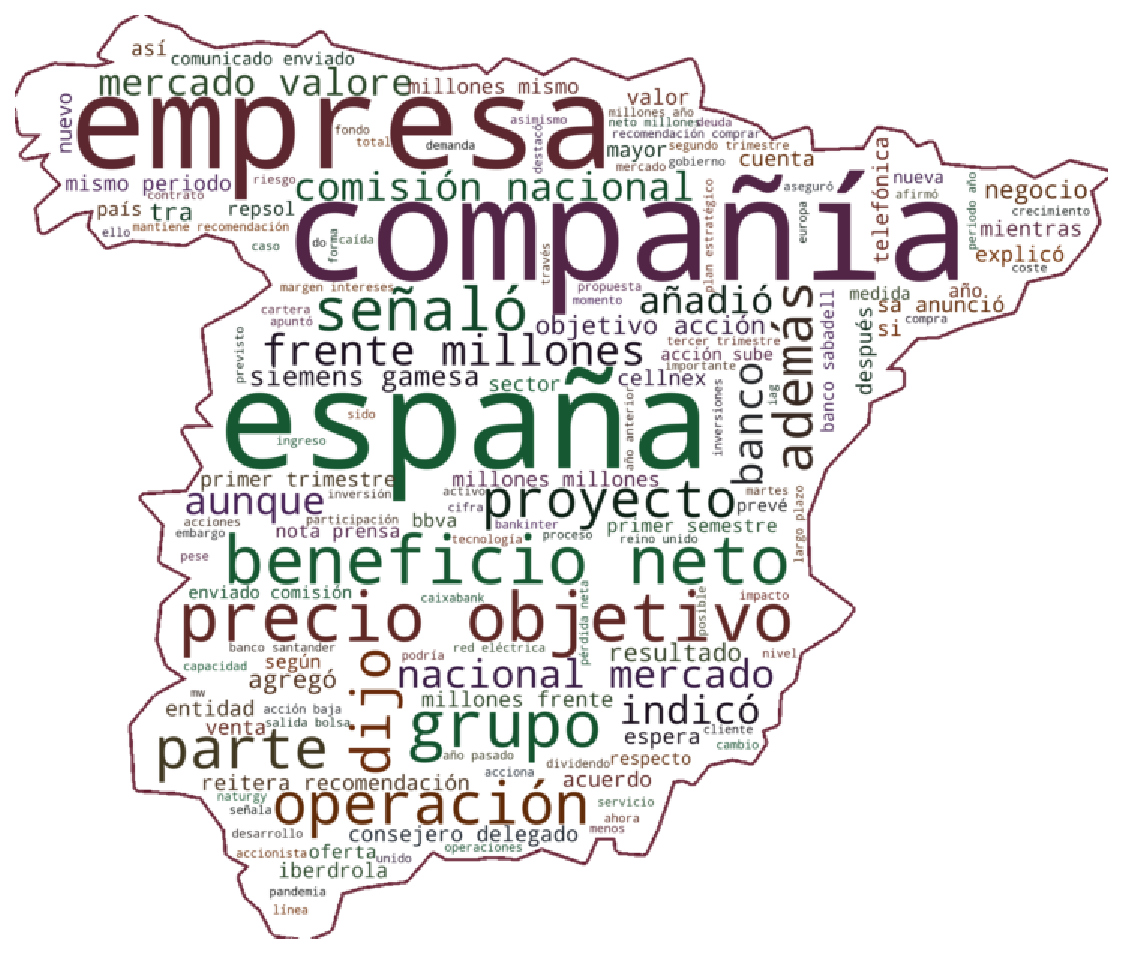
\includegraphics[scale=0.496]{/Users/jesusvillotamiranda/Library/CloudStorage/OneDrive-UniversidaddeLaRioja/CEMFI/__MSc__/__Second_year__/6th_Term/MasterThesis/__Output/EDA_WordCloud.pdf}
  \label{fig:WordCloud}
  \subcaption*{\textit{Note: This Word Cloud visualizes the most frequent words in our dataset of Spanish business news articles. Larger words correspond to higher frequencies. The color of the words is purely for visual differentiation and holds no additional meaning. The most prominent words include \qquote{empresa} (firm), \qquote{compa��a} (company), and \qquote{espa�a} (Spain), reinforcing that the dataset primarily comprises Spanish business news, with a prevalence of technical terms such as \qquote{beneficio neto} (net profit), \qquote{precio objetivo} (target price), \qquote{proyecto} (project), and \qquote{operaci�n} (operation).}}
\end{figure}
%----------------------------------------------------

The distribution of the number of articles published per day is illustrated in \cref{fig:hist_1}, showing that the most frequent publication rate is between 5 and 10 articles per day, though some days exhibit unusually high publication counts. \cref{fig:hist_2} shows the distribution of the number of words per article, with the majority of articles containing between 70 and 280 words. This indicates that the articles are relatively succinct, providing direct information. 
However, the long right tail points to instances of more comprehensive coverage.
%However, a small subset of articles exceeds 500 words, indicating more in-depth coverage.

%----------------------------------------------------
\inserthere{fig:histograms}
\begin{figure}[H]
  \caption{Histogram of \# News Articles per Day and \# Words per Article}
  \centering
  \begin{subfigure}[b]{0.46\textwidth}
    \centering
    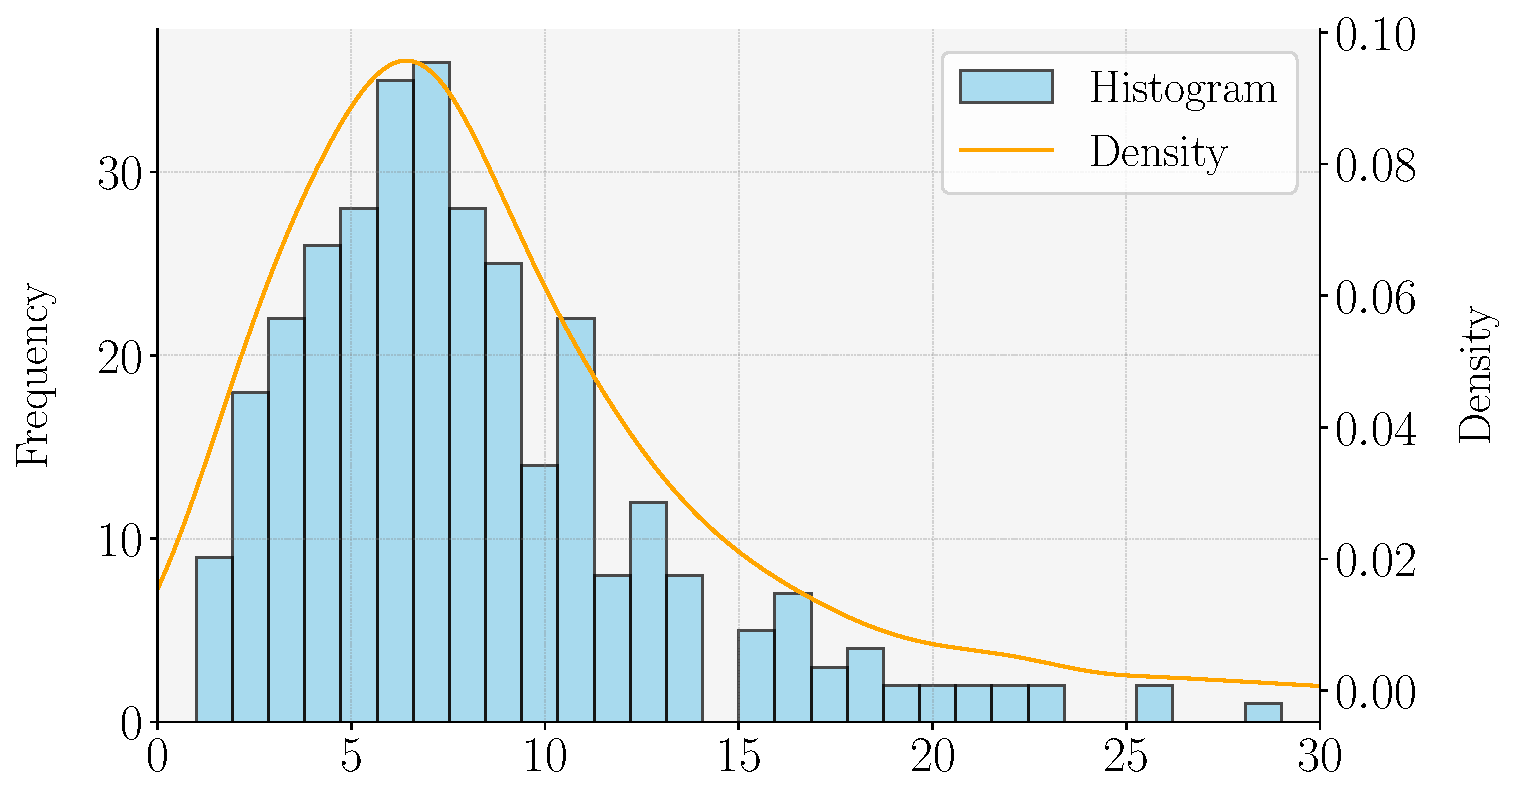
\includegraphics[width=\textwidth]{/Users/jesusvillotamiranda/Library/CloudStorage/OneDrive-UniversidaddeLaRioja/CEMFI/__MSc__/__Second_year__/6th_Term/MasterThesis/__Output/EDA_Histogram_of_Number_of_News_Articles_per_day.pdf}
    \caption{Number of News Articles per Day}
    \label{fig:hist_1}
  \end{subfigure}
  \hspace{0.05\textwidth} % Add horizontal space between the subfigures
  \begin{subfigure}[b]{0.46\textwidth}
    \centering
    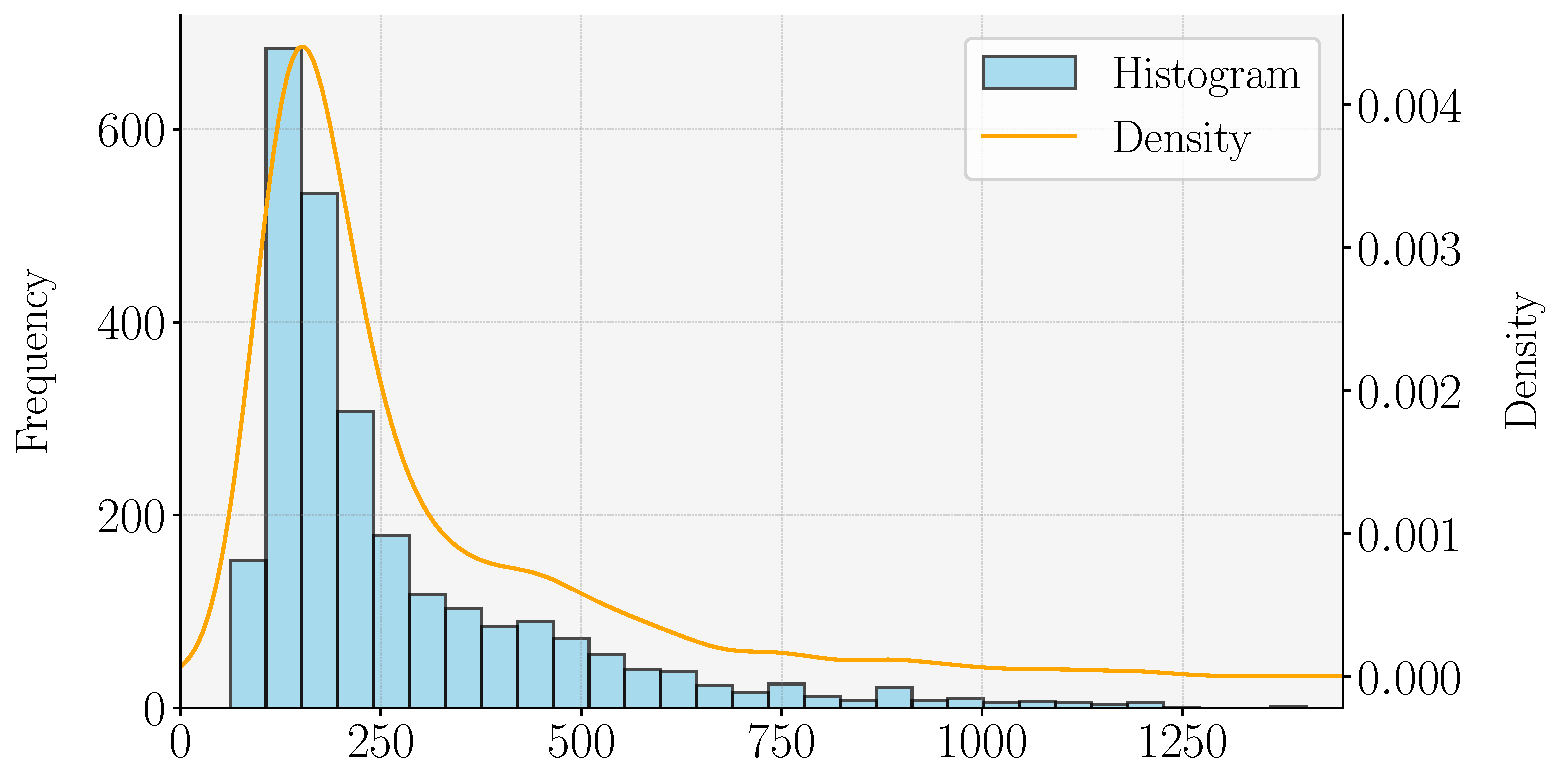
\includegraphics[width=\textwidth]{/Users/jesusvillotamiranda/Library/CloudStorage/OneDrive-UniversidaddeLaRioja/CEMFI/__MSc__/__Second_year__/6th_Term/MasterThesis/__Output/EDA_Number_of_Words_per_Article.pdf}
    \caption{Number of Words per Article}
    \label{fig:hist_2}
  \end{subfigure}
  \label{fig:histograms}
  \subcaption*{\textit{Note: Panel (a) displays the distribution of the number of news articles published per day, with most days having between 5 and 10 articles. Panel (b) shows the distribution of the number of words per article, where the majority are between 70 and 280 words, suggesting concise reporting. However, the long right tail indicates instances of more comprehensive coverage.}}

\end{figure}
%----------------------------------------------------

The time series of the number of articles published per day throughout the sample period is shown in \Cref{fig:ts_articles}. The series exhibits considerable variability, with frequent fluctuations from fewer than 5 articles per day to sudden spikes exceeding 20 articles. The 30-day moving average smooths the series, confirming the previous observation that, on average, between 5 and 10 articles are published daily.

%----------------------------------------------------
\inserthere{fig:ts_articles}
\begin{figure}[H]
  \centering
  \caption{Time Series of Number of Articles per Day and 30-Period Moving Average}
  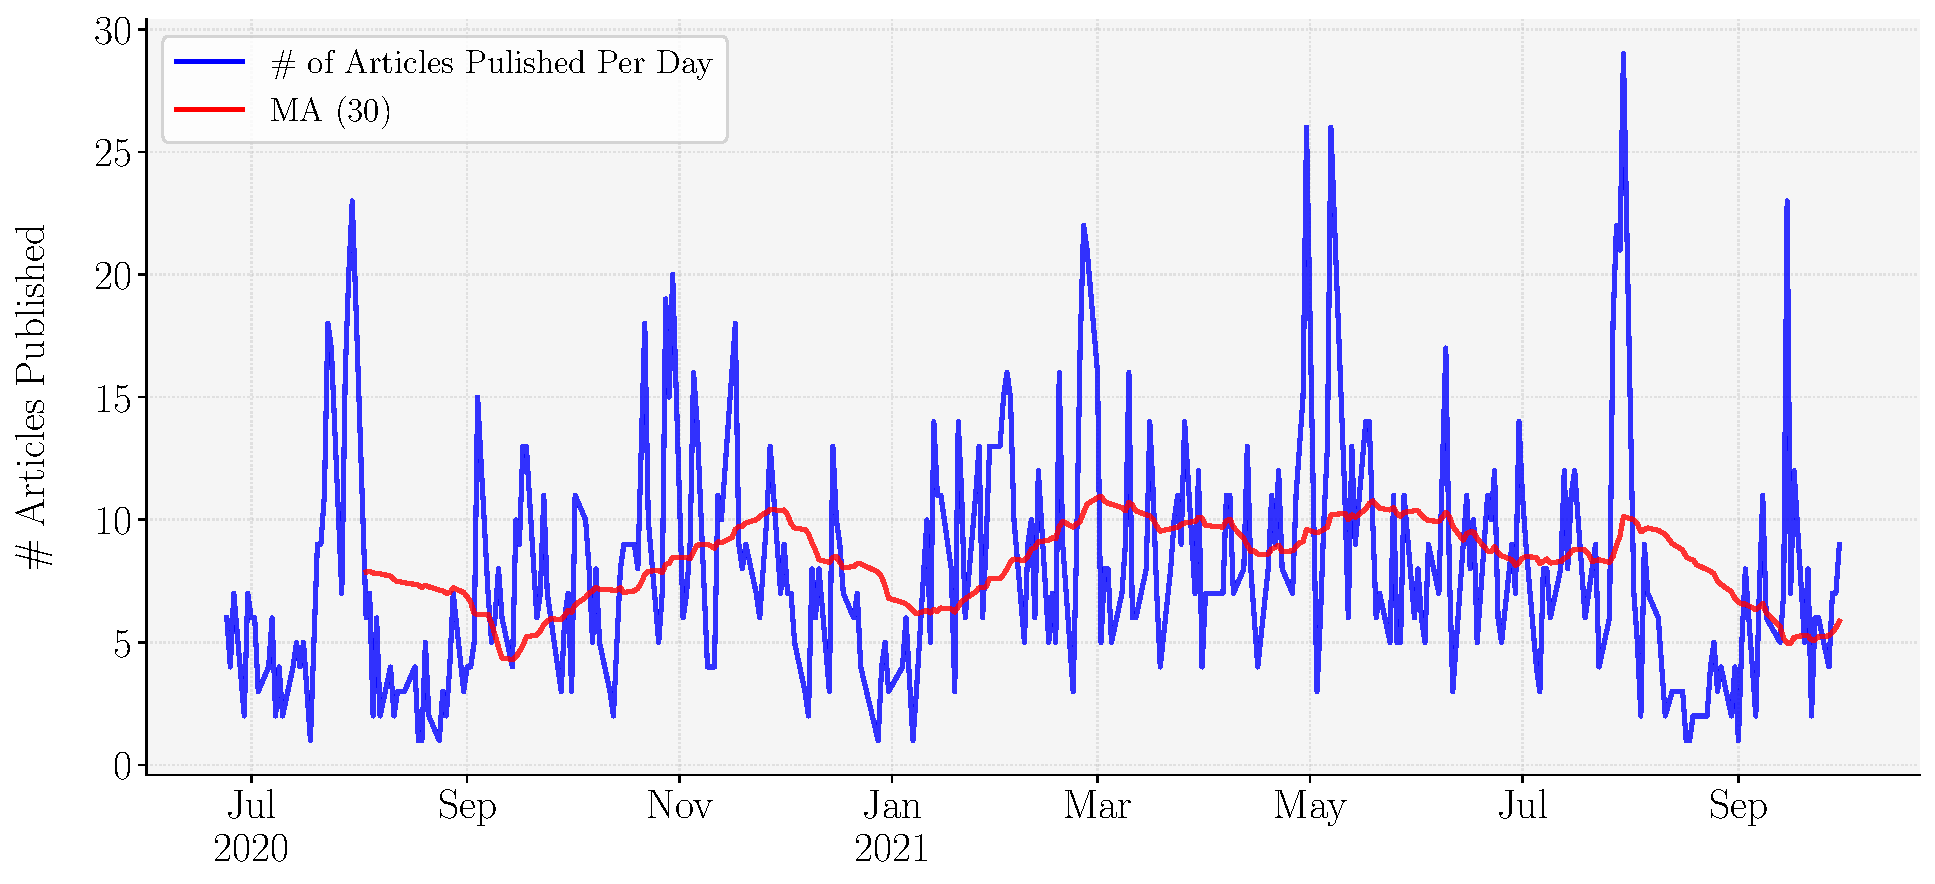
\includegraphics[scale=0.445]{/Users/jesusvillotamiranda/Library/CloudStorage/OneDrive-UniversidaddeLaRioja/CEMFI/__MSc__/__Second_year__/6th_Term/MasterThesis/__Output/EDA_Time_Series_of_Articles.pdf}
  \label{fig:ts_articles}
  \subcaption*{\textit{Note: The time series shows the daily number of news articles published, characterized by significant variability with occasional sharp spikes. The 30-day moving average smooths these fluctuations, revealing an average publication rate of 5 to 10 articles per day.}}
\end{figure}
%----------------------------------------------------

%%%%%%%%%%%%%%%%%% METHODOLOGY %%%%%%%%%%%%%%%%%%%%%%
\section{Methodology}

\subsection{Reinforcement Learning for Asset Pricing}

Reinforcement Learning (RL) is a machine learning paradigm in which an agent interacts with an environment by taking actions, receiving rewards, and updating its policy to maximize long-term cumulative rewards. In the context of asset pricing, the agent represents the model that estimates the SDF and portfolio weights, while the environment is the financial market that provides information about returns, risk factors, and macroeconomic variables.

Formally, the RL framework is defined as a \textit{Markov Decision Process (MDP)}, which consists of the following components:

\subsubsection{State Space ($s_t$)}

The \textit{state space} $s_t$ at time $t$ contains all relevant information needed to price assets and estimate the SDF. In our framework, the state space is composed of:
\[
s_t = \left(I_t, I_{t, i}, \omega_{t-1}, h_t\right)
\]
where:
\begin{itemize}
    \item $I_t$: A vector of macroeconomic variables at time $t$ (e.g., GDP growth, inflation, interest rates).
    \item $I_{t, i}$: A vector of firm-specific characteristics at time $t$ for asset $i$ (e.g., size, book-to-market ratio).
    \item $\omega_{t-1}$: The SDF portfolio weights from the previous time step.
    \item $h_t$: A set of hidden state variables that capture the dynamic patterns in the macroeconomic data, estimated via a Long Short-Term Memory (LSTM) network.
\end{itemize}

The inclusion of $h_t$ allows the model to incorporate both short-term and long-term dependencies in the macroeconomic and firm-specific data. The hidden states $h_t$ are updated at each time step as new macroeconomic information becomes available.

\subsubsection{Action Space ($a_t$)}

At each time step $t$, the agent selects an \textit{action} $a_t$ that adjusts the SDF portfolio weights $\omega_t$ and the risk exposures $\beta_t$. The action space can be either continuous or discrete, depending on the nature of the adjustments. We define the action space as continuous:
\[
a_t = \left(\omega_t, \beta_t\right)
\]
where:
\begin{itemize}
    \item $\omega_t$: The portfolio weights at time $t$ for the SDF.
    \item $\beta_t$: The exposure to systematic risks at time $t$.
\end{itemize}

The goal of the agent is to choose actions that maximize the reward over time, which we define next.

\subsubsection{Reward Function ($R_t$)}

The \textit{reward function} measures the performance of the agent at each time step and is used to guide the learning process. In our framework, the reward function reflects the trade-off between maximizing risk-adjusted returns and minimizing pricing errors. We define the reward function as:
\[
R_t = SR(\omega_t) - \lambda \cdot PE(\omega_t, \beta_t)
\]
where:
\begin{itemize}
    \item $SR(\omega_t)$: The Sharpe ratio of the portfolio with weights $\omega_t$, defined as:
    \[
    SR(\omega_t) = \frac{\mathbb{E}[R_t]}{\sqrt{\operatorname{Var}(R_t)}}
    \]
    where $R_t = \omega_t^\top R_{t+1}^e$ is the portfolio return based on the excess returns $R_{t+1}^e$ of the assets.
    \item $PE(\omega_t, \beta_t)$: The pricing error, which measures the deviation of the model's predicted returns from observed returns, defined as:
    \[
    PE(\omega_t, \beta_t) = \sum_{i=1}^N \left( R_{t+1, i}^e - \beta_{t, i} F_{t+1} \right)^2
    \]
    \item $\lambda$: A regularization parameter that balances the trade-off between maximizing the Sharpe ratio and minimizing the pricing error.
\end{itemize}

The reward function ensures that the agent learns to both optimize portfolio weights for high risk-adjusted returns and minimize the mispricing of assets.

\subsubsection{Policy and Value Functions}

The agent's objective is to learn a policy $\pi(a_t \mid s_t)$ that maps states to actions in a way that maximizes the expected cumulative reward over time:
\[
\pi^* = \arg \max_{\pi} \mathbb{E}\left[\sum_{t=0}^T \gamma^t R_t \mid \pi \right]
\]
where $\gamma \in (0, 1]$ is a discount factor that determines the importance of future rewards. The policy $\pi$ is typically parameterized by a neural network, and the optimization is done using a gradient-based method such as \textit{policy gradient} or \textit{Deep Q-Learning}.

The policy is updated iteratively as the agent interacts with the market environment. At each time step, the agent observes the current state $s_t$, selects an action $a_t$ based on the current policy, and receives a reward $R_t$. The policy is then updated to improve the expected cumulative reward.

\subsubsection{Actor-Critic Architecture}

We adopt an \textit{actor-critic} architecture to implement the RL model:
\begin{itemize}
    \item The \textbf{actor} network represents the policy $\pi(s_t)$ and outputs the action $a_t = \{ \omega_t, \beta_t \}$.
    \item The \textbf{critic} network estimates the value function $V^\pi(s_t)$ and evaluates the quality of the current state-action pair.
\end{itemize}

The critic network helps the actor update its policy by providing feedback on the long-term value of the actions taken. This structure allows for continuous improvement of the policy over time.

\subsection{LSTM for Macroeconomic Dynamics}

Macroeconomic variables are often non-stationary and exhibit complex dynamic patterns. To capture these dynamics, we use a \textit{Long Short-Term Memory (LSTM)} network to estimate hidden state variables $h_t$ that summarize the information in the macroeconomic time series. The LSTM processes the sequence of macroeconomic observations $\left(I_0, I_1, \ldots, I_t\right)$ and outputs a hidden state $h_t$ that reflects both short-term and long-term dependencies.

Formally, the LSTM updates the hidden state according to the following equations:
\[
h_t = \sigma\left(W_h h_{t-1} + W_x I_t + b_h \right)
\]
where $\sigma$ is a non-linear activation function, $W_h$ and $W_x$ are weight matrices, and $b_h$ is a bias term. The hidden state $h_t$ is then used as an input to the RL agent for making decisions about portfolio adjustments.

\subsection{GAN and Reinforcement Learning Integration}

In our model, we integrate the \textit{Generative Adversarial Network (GAN)} from \textit{Chen, Pelger, and Zhu (2023)} into the RL framework. The adversarial network in GAN selects the hardest-to-price moments, and the RL agent learns to adjust the portfolio weights and risk exposures to minimize the worst-case pricing errors. The GAN serves as the environment, continually presenting challenges for the RL agent to solve.

At each step, the RL agent interacts with the GAN by selecting portfolio weights $\omega_t$ and risk loadings $\beta_t$, and the GAN adversary responds by identifying the moments where pricing errors are largest. The RL agent then updates its policy based on the reward function, adjusting its actions to minimize these errors and maximize the Sharpe ratio.


%%%%%%%%%%%%%%% EMPRICAL APPLICATION %%%%%%%%%%%%%%%%%
\section{Empirical Application}
%----------------------------------------------------
\subsection{Assumptions}
To ensure transparency in our empirical analysis, we explicitly outline the critical assumptions underlying the implementation of our proposed pairs trading strategy. These assumptions reflect idealized market conditions necessary for theoretical feasibility and reproducibility of results.
%To be transparent about the procedures implemented in this application, we need to set forward a set of assumptions that are crucial for the feasibility of the proposed trading strategy and to obtain our results.


\begin{assumption}[Price Execution] \label{assum:execution}
All trades are executed at daily adjusted closing prices. This assumption requires sufficient market liquidity and depth to accommodate position entries and exits without significant price impact or execution delays.
\end{assumption}

\begin{assumption}[Short Selling Access] \label{assum:shorting}
Unrestricted short selling is permitted for all assets, including the ability to maintain leveraged short positions. This encompasses having reliable access to securities lending facilities and the capacity to meet associated margin requirements.
\end{assumption}

\begin{assumption}[Leverage Capacity] \label{assum:leverage}
Trading positions can employ substantial leverage on both long and short sides. This assumes access to margin facilities that permit position sizes meaningfully larger than the allocated capital base, subject to prevailing broker and regulatory requirements.
%Investors may employ leveraged positions up to a 200:1 leverage factor. This allows increasing exposure to mispricing opportunities but amplifies potential losses.
%Trading positions can be leveraged up to 4:1 on both long and short sides. This leverage constraint aligns with standard margin requirements for US equity trading while maintaining reasonable risk management practices.
\end{assumption}

%\begin{assumption}
%Trades are executed at (adjusted) closing prices (this implicitly embeds assumptions about the liquidity of the traded assets and the order of their trade book).
%\end{assumption}
%
%\begin{assumption}
%High leverage positionsa are allowed (specify leverage factor).
%\end{assumption}
%
%\begin{assumption}
%Short selling and leveraged short selling is allowed.
%\end{assumption}

While these assumptions may appear restrictive, recent developments in financial technology and market structure have made such trading conditions increasingly accessible. Modern electronic trading platforms like Alpaca, Interactive Brokers, and similar services now offer retail investors sophisticated capabilities previously reserved for institutional traders. These platforms provide programmatic trading interfaces, competitive margin rates, and extensive short-selling facilities that may align with our implementation requirements.


%==============[	  CAUTION PARAGRAPH  ]==============
\textbf{Cautionary note.} \textit{This paper is intended for academic and informational purposes only and does not constitute financial advice. The strategies and methodologies discussed involve significant risks, including the potential loss of capital. Past performance is not indicative of future results, and the authors assume no liability for decisions made by individuals or entities based on the content of this research. Readers are advised to consult qualified financial professionals before engaging in trading activities.}
%----------------------------------------------------





%%%%%%%%%%%%%%%%%% CONCLUSION %%%%%%%%%%%%%%%%%%%%%%
%%----------------------------------------------------
\section{Conclusion}
%----------------------------------------------------
%\hspace{0.5cm} 
This paper investigates how information from business news affects stock market prices. We analyze a dataset of Spanish business articles during a particularly volatile period-the COVID-19 pandemic-and examine firm-specific stock market reactions to news. We show that transforming text into vector embeddings and clustering them using KMeans yields clusters that are firm-specific and industry-specific. However, the distribution of articles across clusters is unstable over sequential data splits, indicating temporal instability. When we implement a cluster-based trading strategy-similar to portfolio sorts-on the KMeans clusters, we observe an over-reliance on the past performance of a cluster. That is, signals are short-lived due to temporal instability. Consequently, the out-of-sample profitability of the trading strategy is negligible, evidencing the method's poor temporal generalizability. Therefore, a model based on embeddings is superficial and is not able to anticipate market trends.

%----------------------------------------------------
Alternatively, we develop a novel approach by guiding a Large Language Model (LLM) through a structured news-parsing schema, enabling it to analyze news-implied firm-specific economic shocks. The schema involves identifying the firms affected by the articles and classifying the implied shocks on such firms by their type, magnitude, and direction. This LLM-based methodology demonstrates several advantages over the traditional clustering approach. Even in a volatile period, it produces stable distributions of articles across clusters in sequential splits, demonstrating robust temporal stability. Moreover, the resulting trading signals are both long-lasting and economically relevant, as they are based on fundamental economic shocks rather than statistical patterns. The results show that the LLM-based trading strategy effectively identifies winners and losers, illustrating the parser's ability to anticipate market trends by comprehending the economic implications of firm-specific shocks. This approach generates a consistent profile of earnings in the test set, with results robust to the choice of hyperparameters-the holding period length of the trading strategy and the number of selected clusters for trading. Our findings demonstrate a promising avenue: LLMs, when guided by appropriate economic frameworks, can help predict market reactions to news through systematic classification of economic shocks embedded in financial narratives.


%%%%%%%%%%%%%%%%%% BIBLIOGRAPHY %%%%%%%%%%%%%%%%%%%%%%
\bibliography{bib_references_DOI.bib}
\bibliographystyle{plain}

%----------------------------------------------------
%\newpage
%% To make sure all the tables/figures appear before the appendix
%\processdelayedfloats 
% Reset the numbering for appendix figures and tables
%\renewcommand{\thefigure}{A\arabic{figure}} 
%\renewcommand{\thetable}{A\arabic{table}}
%----------------------------------------------------

%%%%%%%%%%%%%%%%%%% APPENDIX %%%%%%%%%%%%%%%%%%%%%%
\appendix
\section{Online Appendix}
\subsection{KMeans Algorithm}
%----------------------------------------------------
% Alternative 1: Algorithmic Setup
\begin{algorithm}[H]
\caption{KMeans Clustering Algorithm}
\label{alg:KMeans}
\begin{algorithmic}[1]
\State \textbf{Input:} Embedding vectors $\{\mathbf{e}^1, \mathbf{e}^2, \ldots, \mathbf{e}^{N}\}$, number of clusters $k$
\State \textbf{Output:} Cluster assignments $\{\D_1, \D_2, \ldots, \D_k\}$, centroids $\{\mathbf{c}_1, \mathbf{c}_2, \ldots, \mathbf{c}_k\}$

\State \textbf{Initialize} centroids $\{\mathbf{c}_1, \mathbf{c}_2, \ldots, \mathbf{c}_k\}$ randomly

\Repeat
    \State \underline{\textit{Assignment Step:}}
    \For{each vector $\mathbf{e}^i$}
        \State Assign $\mathbf{e}^i$ to the nearest centroid:
        \[
        g = \arg \min_{\ell\in\{1,...,k\}} \|\mathbf{e}^i - \mathbf{c}_{\ell}\|_{2}^2
        \]
        \State Update cluster assignments: $\D_{g} \leftarrow \D_{g} \cup \{i\}$
    \EndFor

    \State \underline{\textit{Update Step:}}
    \For{each cluster $\D_g$}
        \State Recalculate centroid $\mathbf{c}_g$:
        \[
        \mathbf{c}_g = \frac{1}{|\D_g|} \sum_{i \in \D_g} \mathbf{e}^i
        \]
    \EndFor
\Until{cluster assignments no longer change}

\State \textbf{Return} cluster assignments $\{\D_1, \D_2, \ldots, \D_k\}$ and centroids $\{\mathbf{c}_1, \mathbf{c}_2, \ldots, \mathbf{c}_k\}$

\end{algorithmic}
\end{algorithm}

%----------------------------------------------------
% Alternative 2: More organized setup
%\section*{KMeans Clustering Algorithm}

\subsection*{Inputs}
\begin{itemize}
    \item Embedding vectors: $\{\mathbf{e}^1, \mathbf{e}^2, \ldots, \mathbf{e}^{N_{tr}}\}$
    \item Number of clusters: $k$
\end{itemize}

\subsection*{Outputs}
\begin{itemize}
    \item Cluster assignments: $\{C_1, C_2, \ldots, C_k\}$
    \item Centroids: $\{\mathbf{c}_1, \mathbf{c}_2, \ldots, \mathbf{c}_k\}$
\end{itemize}

\subsection*{Algorithm}
\begin{enumerate}
    \item \textbf{Initialize} centroids $\{\mathbf{c}_1, \mathbf{c}_2, \ldots, \mathbf{c}_k\}$ randomly.
    \item \textbf{Repeat until convergence:}
    \begin{enumerate}
        \item \textbf{Assignment Step:}
        \[
        C_j = \left\{ \mathbf{e}^i \mid j = \arg \min_{l} \|\mathbf{e}^i - \mathbf{c}_l\|^2, \quad l = 1, 2, \ldots, k \right\}
        \]
        \item \textbf{Update Step:}
        \[
        \mathbf{c}_j = \frac{1}{|C_j|} \sum_{\mathbf{e}^i \in C_j} \mathbf{e}^i, \quad \forall j = 1, 2, \ldots, k
        \]
    \end{enumerate}
    \item \textbf{Convergence Criterion:} Repeat steps 2(a) and 2(b) until the cluster assignments do not change, i.e.,
    \[
    C_j^{(t+1)} = C_j^{(t)}, \quad \forall j = 1, 2, \ldots, k
    \]
    where $t$ denotes the iteration number.
\end{enumerate}

\subsection*{Objective}
The KMeans algorithm aims to minimize the within-cluster sum of squares (WCSS):
\[
\min_{C, \mathbf{c}} \sum_{j=1}^k \sum_{\mathbf{e}^i \in C_j} \|\mathbf{e}^i - \mathbf{c}_j\|^2
\]


%----------------------------------------------------

\newpage
%%%%%%%%%%%%%%%%%%%%%%%%%%%%%%%%%%%%%%%%%%%%%%%%%%%%%
\subsection{Hyperparameter Choice}
Our hyperparameters are $L$ and $\theta$. Recall that $L$ denotes the number of trading days over which we hold the positions in the beta-neutral strategy, while $\theta$ represents the upper bound on each side (long and short) for the amount of clusters we select for the trading strategy. The specific choice of hyperparameters we made for the results presented in the paper were:
\begin{align*}
L &= 4
\\
\theta &= \integer{0.5k}
\end{align*}
where $k$ represents the number of clusters (26 for KMeans clustering, and 20 for LLM clustering). This choice is not arbitrary nor opportunistic. Instead, it results from the maximization of the Sharpe Ratio of the portfolio in the train and validation samples for both KMeans and LLM clustering. This choice procedure is completely based on \textit{in-sample} criteria and it prevents lookahead bias. The justification for such choices is made below.

\subsubsection{KMeans Clustering}

In \cref{fig:KMeans_hyperparameter_justification_L} we can see that a choice of $L=4$ in the training and validation splits generates the most stable Sharpe Ratio. Namely, In the train set (\cref{fig:K_hyp_1}), it makes more sense to choose low values of $L$ (less than 4) to maximize the $SR$. However, in the validation set (\cref{fig:K_hyp_2}), it makes more sense to choose higher values of $L$. The choice of $L=4$ represents a balanced compromise, providing a stable Sharpe Ratio profile across both splits, ensuring consistent in-sample performance.
%The choice of $L=4$ stands as a middle ground between this contradiction, generating a stable choice and a stable profile of earnings in sample.

%----------------------------------------------------
\inserthere{fig:KMeans_hyperparameter_justification_L}
\begin{figure}[H]
  \caption{Sharpe Ratios in the train and validation splits as a function of $L$ (KMeans)}
  \centering
  
  \begin{subfigure}[b]{0.46\textwidth}
    \centering
    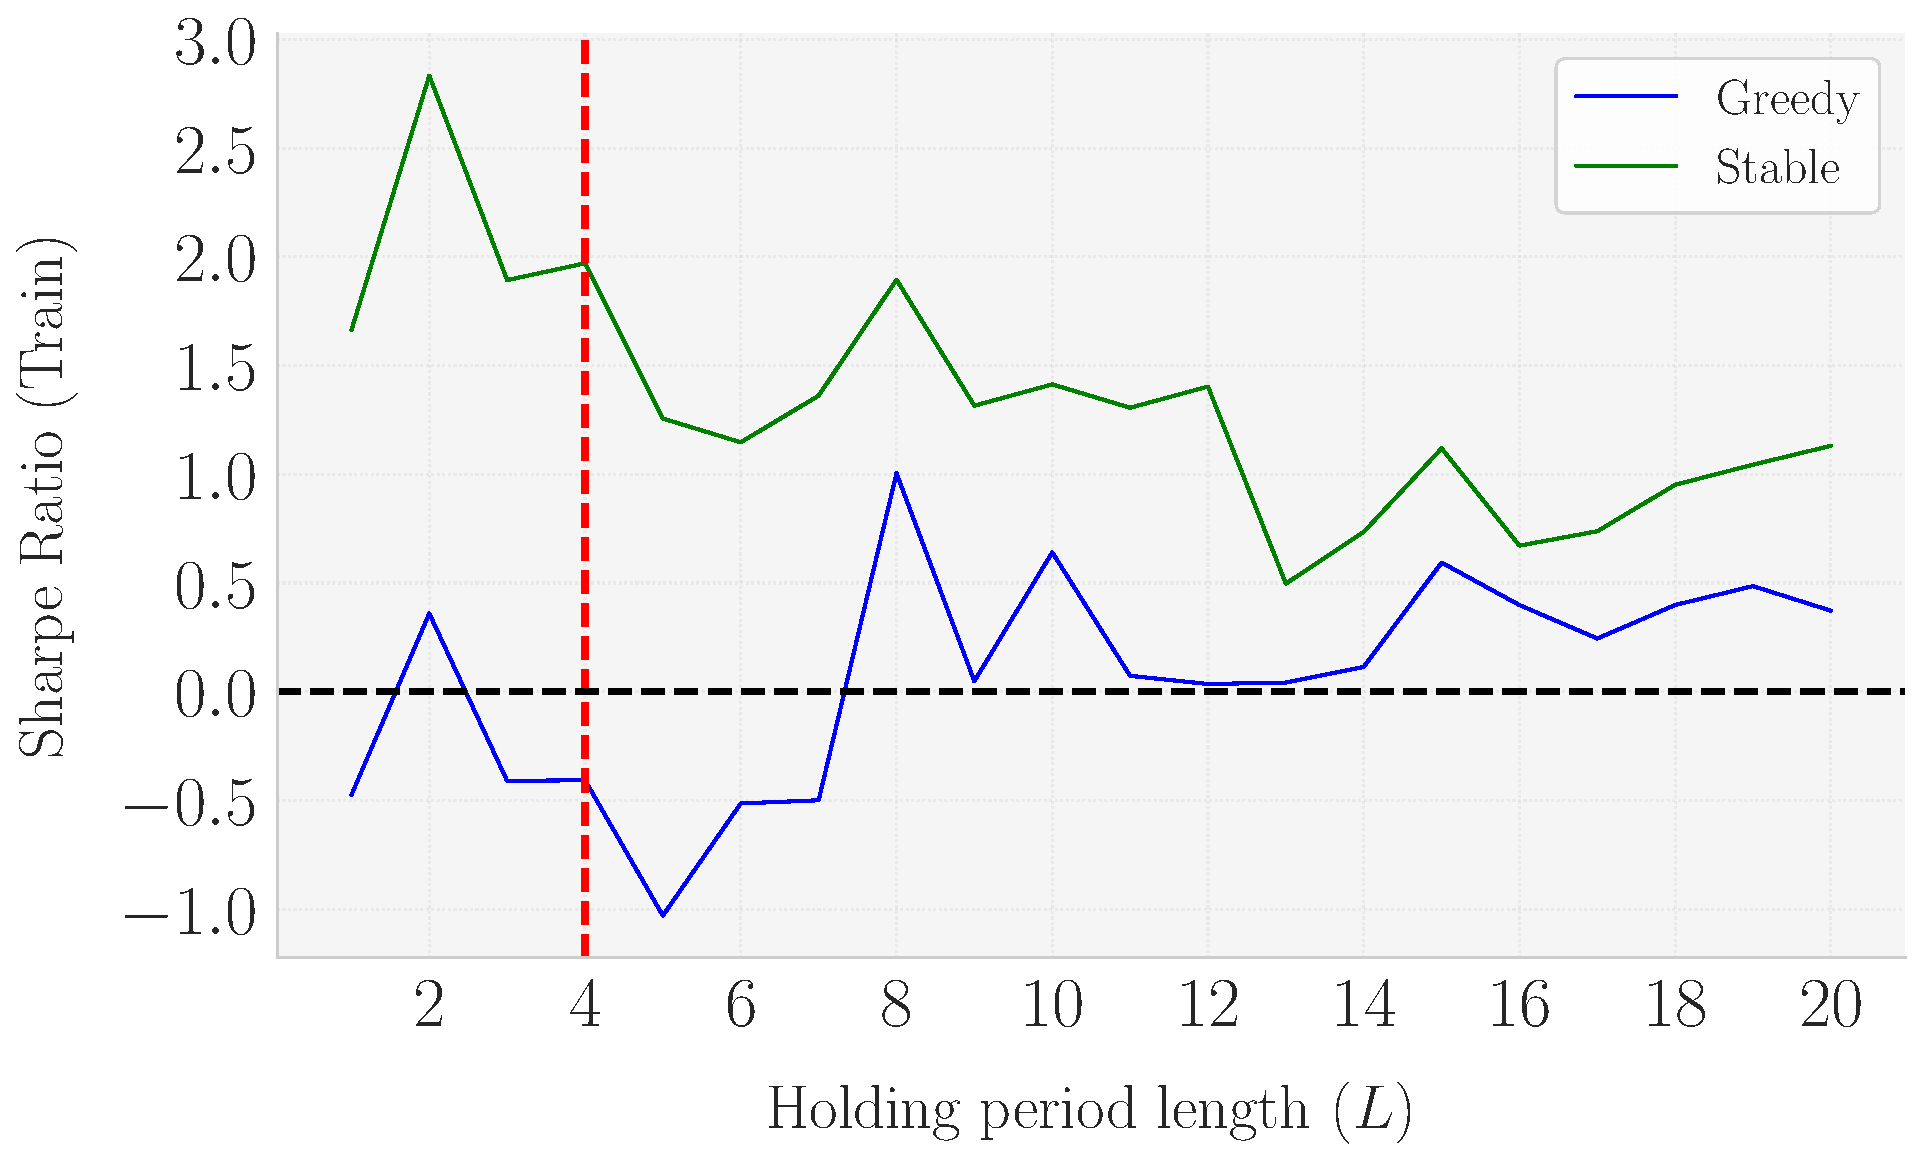
\includegraphics[width=\textwidth]{/Users/jesusvillotamiranda/Library/CloudStorage/OneDrive-UniversidaddeLaRioja/CEMFI/__MSc__/__Second_year__/6th_Term/MasterThesis/__Output/KMeans_RobustnessCheck_SR_Train_Set_vs_L_[Change_L].pdf}
    \caption{Plot of $SR^{\mathcal P^{tr}}(L)$ over a grid of $L$}
    \label{fig:K_hyp_1}
  \end{subfigure}
  \hspace{0.05\textwidth} % Add horizontal space between the subfigures
  \begin{subfigure}[b]{0.46\textwidth}
    \centering
    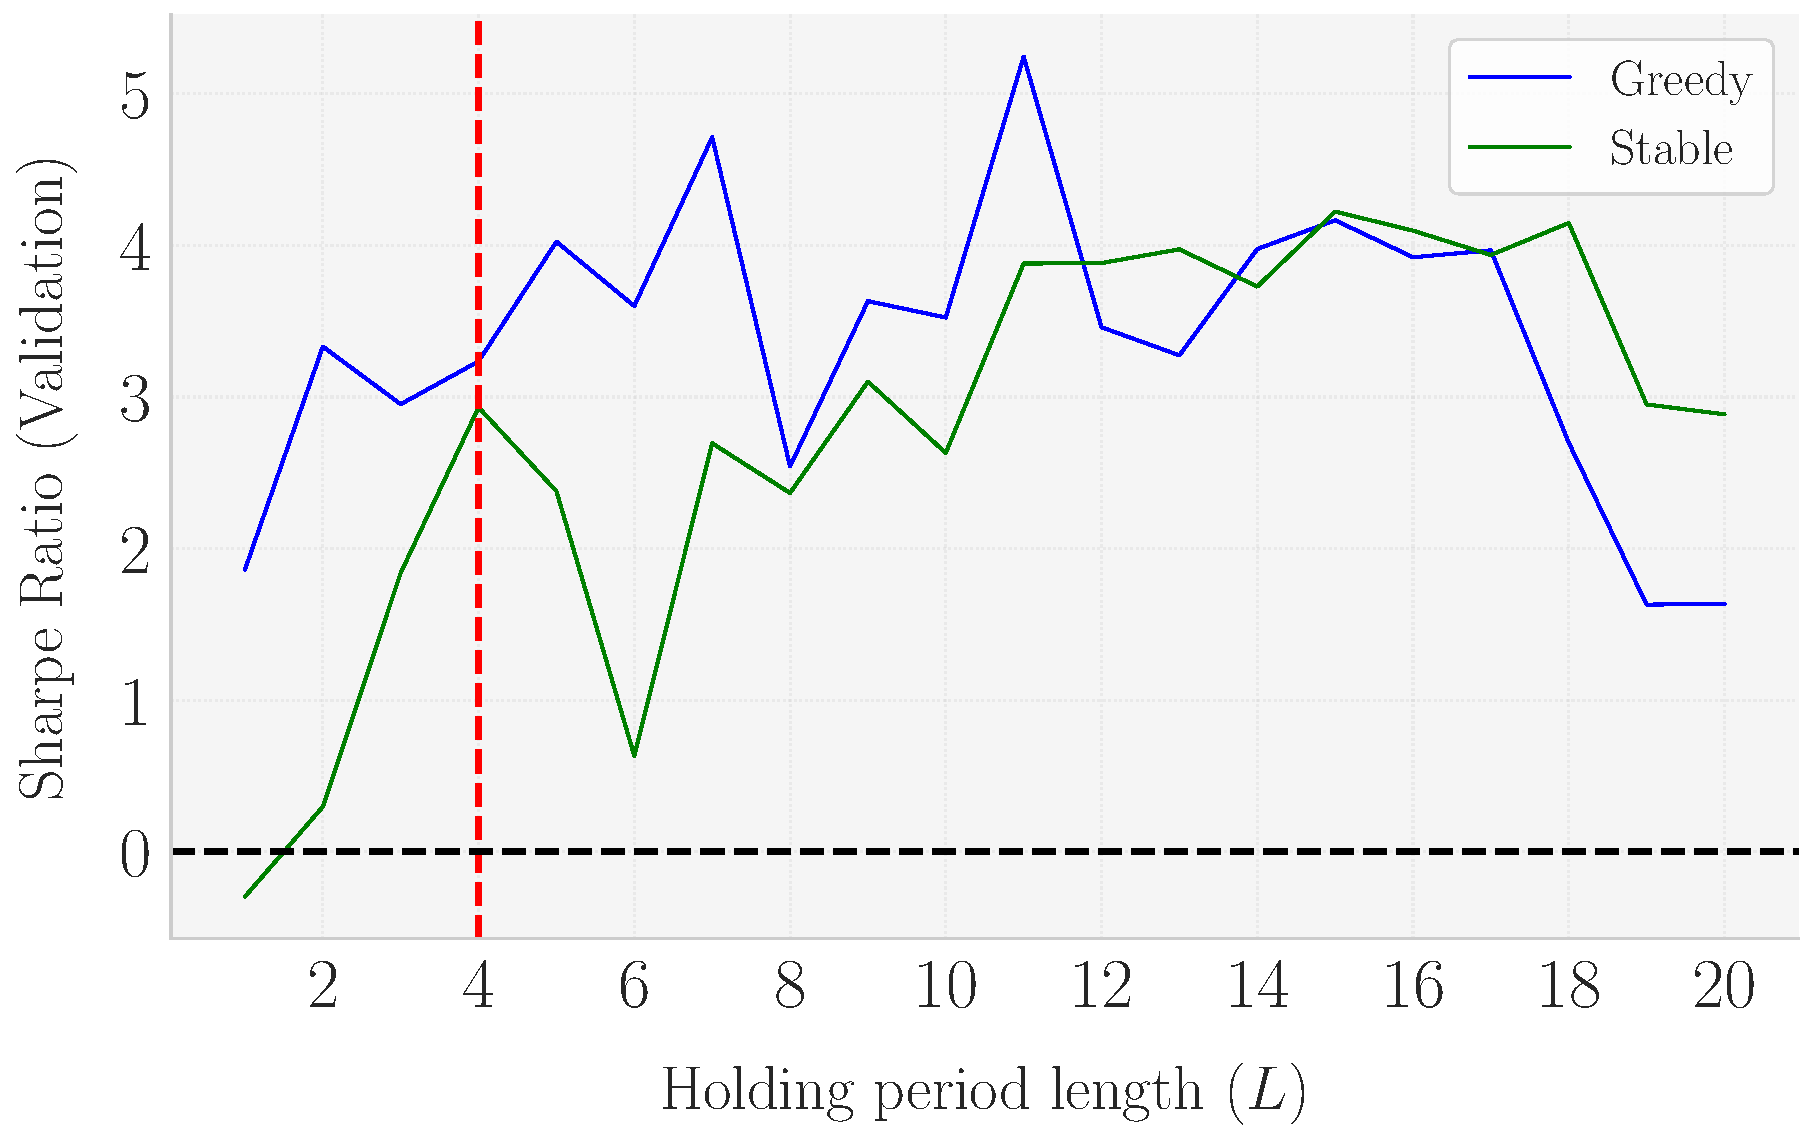
\includegraphics[width=\textwidth]{/Users/jesusvillotamiranda/Library/CloudStorage/OneDrive-UniversidaddeLaRioja/CEMFI/__MSc__/__Second_year__/6th_Term/MasterThesis/__Output/KMeans_RobustnessCheck_SR_Validation_Set_vs_L_[Change_L].pdf}
    \caption{Plot of $SR^{\mathcal P^{val}}(L)$ over a grid of $L$}
    \label{fig:K_hyp_2}
  \end{subfigure}  
  \mx
  \subcaption*{\textit{Note: This figure shows the Sharpe Ratios ($SR$) as a function of the holding period length ($L$) for the KMeans clustering method in the training (Panel a) and validation (Panel b) splits. In Panel (a), the Sharpe Ratios in the training set indicate that lower values of $L$ (less than 4) maximize performance. Conversely, in Panel (b), the validation set shows higher Sharpe Ratios for longer holding periods. The choice of $L=4$ represents a balanced compromise, providing a stable Sharpe Ratio profile across both splits, ensuring consistent in-sample performance without introducing lookahead bias.}}
  \label{fig:KMeans_hyperparameter_justification_L}
\end{figure}
%----------------------------------------------------

On the other hand, the choice of $\theta=\integer{0.5\cd 26}=13$ is a choice that pursues stability in the Sharpe Ratio of the train and validation portfolios. As we can see from \cref{fig:KMeans_hyperparameter_justification_theta}, the Sharpe Ratios tend to converge to the highest and most stable value when we choose the highest possible value of $\theta$. 

 %----------------------------------------------------
\inserthere{fig:KMeans_hyperparameter_justification_theta}
\begin{figure}[H]
  \caption{Sharpe Ratios in the train and validation splits as a function of $\theta$ (KMeans)}
  \centering
    \begin{subfigure}[b]{0.46\textwidth}
    \centering
    \includegraphics[width=\textwidth]{/Users/jesusvillotamiranda/Library/CloudStorage/OneDrive-UniversidaddeLaRioja/CEMFI/__MSc__/__Second_year__/6th_Term/MasterThesis/__Output/KMeans_RobustnessCheck_SR_Train_Set_vs_theta_[Change_theta].pdf}
    \caption{Plot of $SR^{\mathcal P^{tr}}(\theta)$ over a grid of $\theta$}
    \label{fig:K_hyp_3}
  \end{subfigure}
  \hspace{0.05\textwidth} % Add horizontal space between the subfigures
  \begin{subfigure}[b]{0.46\textwidth}
    \centering
    \includegraphics[width=\textwidth]{/Users/jesusvillotamiranda/Library/CloudStorage/OneDrive-UniversidaddeLaRioja/CEMFI/__MSc__/__Second_year__/6th_Term/MasterThesis/__Output/KMeans_RobustnessCheck_SR_Validation_Set_vs_theta_[Change_theta].pdf}
    \caption{Plot of $SR^{\mathcal P^{val}}(\theta)$ over a grid of $\theta$}
    \label{fig:K_hyp_4}
  \end{subfigure}
  \mx
\subcaption*{\textit{Note: This figure illustrates the Sharpe Ratios ($SR$) as a function of $\theta$, the upper bound on the number of traded clusters, for the KMeans clustering method in the training (Panel a) and validation (Panel b) splits. In Panel (a), the Sharpe Ratios in the training set show a trend of increasing stability and maximizing performance as $\theta$ approaches its upper limit. Similarly, Panel (b) displays a consistent pattern in the validation set, where higher values of $\theta$ lead to convergence at the highest and most stable Sharpe Ratios. The choice of $\theta = 13$ (i.e: $\integer{0.5 \cdot 26}$) reflects this observed stability and optimization, providing a balanced and robust selection for the portfolio strategy.}}
  \label{fig:KMeans_hyperparameter_justification_theta}
\end{figure}
%----------------------------------------------------


\subsubsection{LLM Clustering}
Following a similar logic as below, the choice of $L=4$ sets a consensus between the maximization of $SR^{\mathcal P^{tr}}$ and $SR^{\mathcal P^{val}}$. That is, maximizing $SR^{\mathcal P^{tr}}$ requires lower holding period lengths (the maximizer is $L=4$), while maximizing $SR^{\mathcal P^{val}}$ requires increasing the window length. Among this contradiction, $L=4$ standing as a perfect choice to balance the maximization requirements in both samples, generating a stable choice for the holding period window length.

%----------------------------------------------------
\inserthere{fig:LLM_hyperparameter_justification_L}
\begin{figure}[H]
  \caption{Sharpe Ratios in the train and validation splits as a function of hyperparameters (LLM)}
  \centering
  
  \begin{subfigure}[b]{0.46\textwidth}
    \centering
    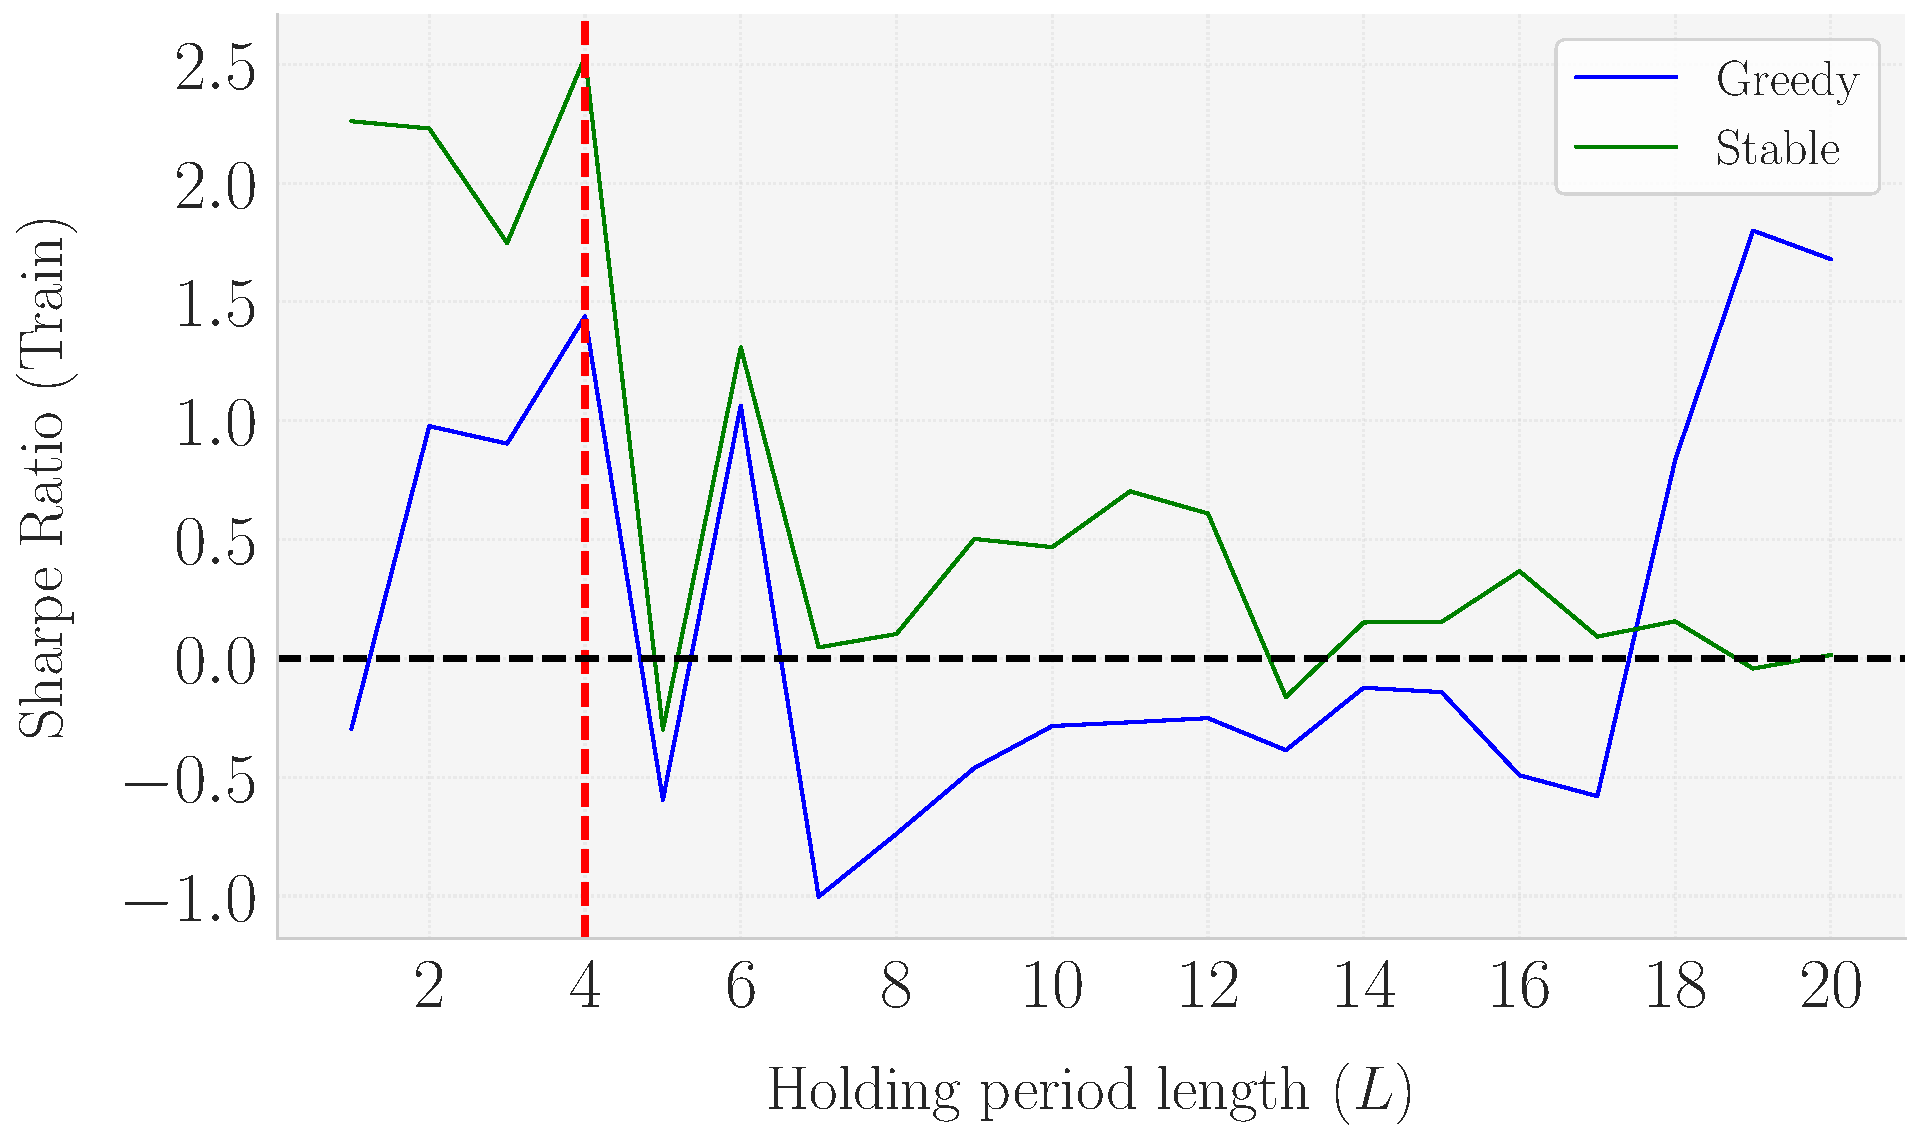
\includegraphics[width=\textwidth]{/Users/jesusvillotamiranda/Library/CloudStorage/OneDrive-UniversidaddeLaRioja/CEMFI/__MSc__/__Second_year__/6th_Term/MasterThesis/__Output/LLAMA_RobustnessCheck_SR_Train_Set_vs_L_[Change_L].pdf}
    \caption{Plot of $SR^{\mathcal P^{tr}}(L)$ over a grid of $L$}
    \label{fig:LLM_hyp_1}
    
  \end{subfigure}
  \hspace{0.05\textwidth} % Add horizontal space between the subfigures
  \begin{subfigure}[b]{0.46\textwidth}
    \centering
    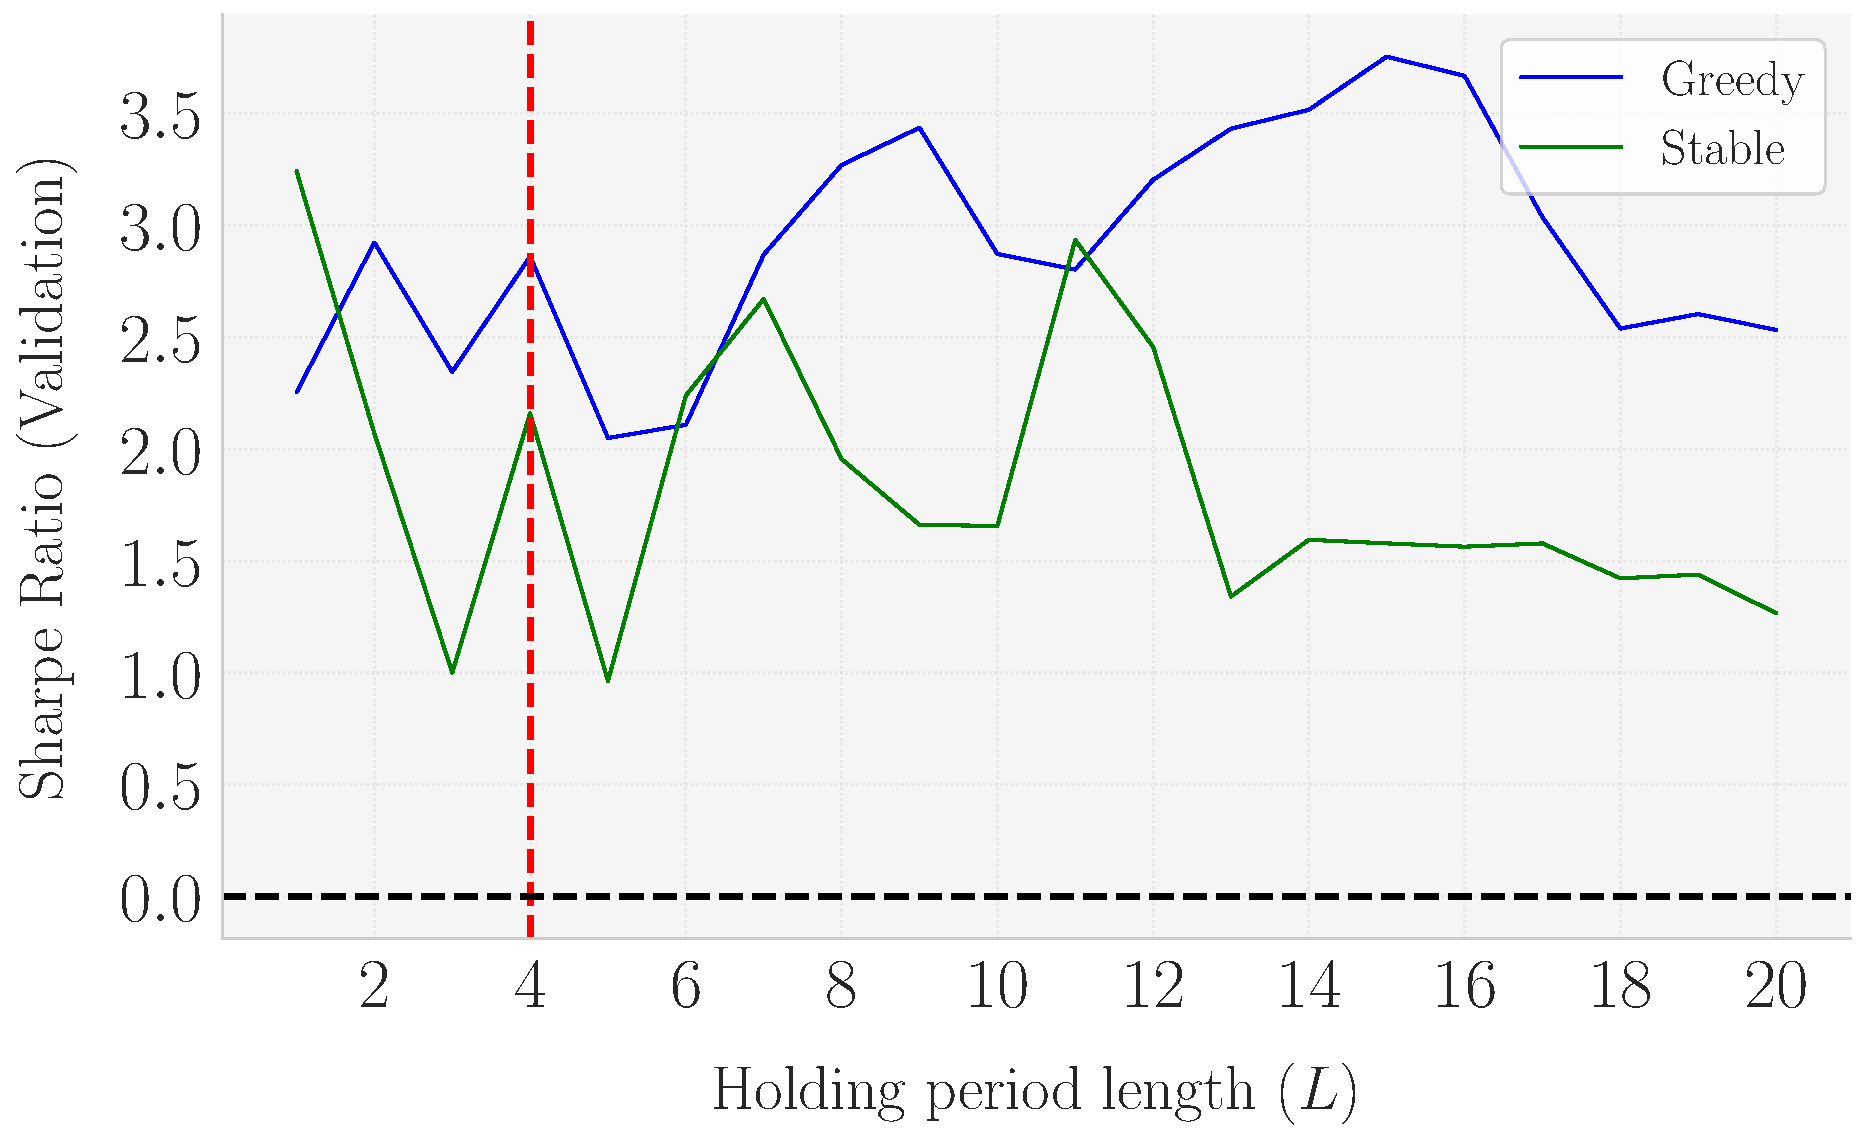
\includegraphics[width=\textwidth]{/Users/jesusvillotamiranda/Library/CloudStorage/OneDrive-UniversidaddeLaRioja/CEMFI/__MSc__/__Second_year__/6th_Term/MasterThesis/__Output/LLAMA_RobustnessCheck_SR_Validation_Set_vs_L_[Change_L].pdf}
    \caption{Plot of $SR^{\mathcal P^{val}}(L)$ over a grid of $L$}
    \label{fig:LLM_hyp_2}
  \end{subfigure}
  \mx 
  \subcaption*{\textit{Note: This figure shows the Sharpe Ratios ($SR$) as a function of the holding period length ($L$) for the LLM clustering method, across the training (Panel a) and validation (Panel b) splits. In Panel (a), the Sharpe Ratios in the training set reach their maximum at $L=4$, suggesting shorter holding periods are more effective for maximizing performance. Conversely, Panel (b) illustrates that longer holding periods yield higher Sharpe Ratios in the validation set. The choice of $L=4$ serves as a compromise, balancing the trade-off between maximizing $SR$ in both splits and providing a stable and consistent holding period length for the strategy.}}
  \label{fig:LLM_hyperparameter_justification_L}
\end{figure}
%----------------------------------------------------

Finally, the same conclusion as in KMeans applies here. By selecting $\theta=\integer{0.5\cd 20}=10$, we get a stable Sharpe Ratio. Even though we observe that $SR^{\mathcal P^{tr}}(L)$ falls momentarily at $\theta=10$ for the Greedy algorithm, it still constitutes a good choice. Conversely, at $\theta=10$ the greedy algorithm sees a jump in $SR^{\mathcal P^{val}}(L)$. All in all, we can easily conclude that $\theta=\integer{0.5k}$ arises as a good hyperpamrameter choice also for LLM clustering.
%----------------------------------------------------
\inserthere{fig:LLM_hyperparameter_justification_theta}
\begin{figure}[H]
\caption{Sharpe Ratios in the train and validation splits as a function of $\theta$ (LLM)}
  \centering

    \begin{subfigure}[b]{0.46\textwidth}
    \centering
    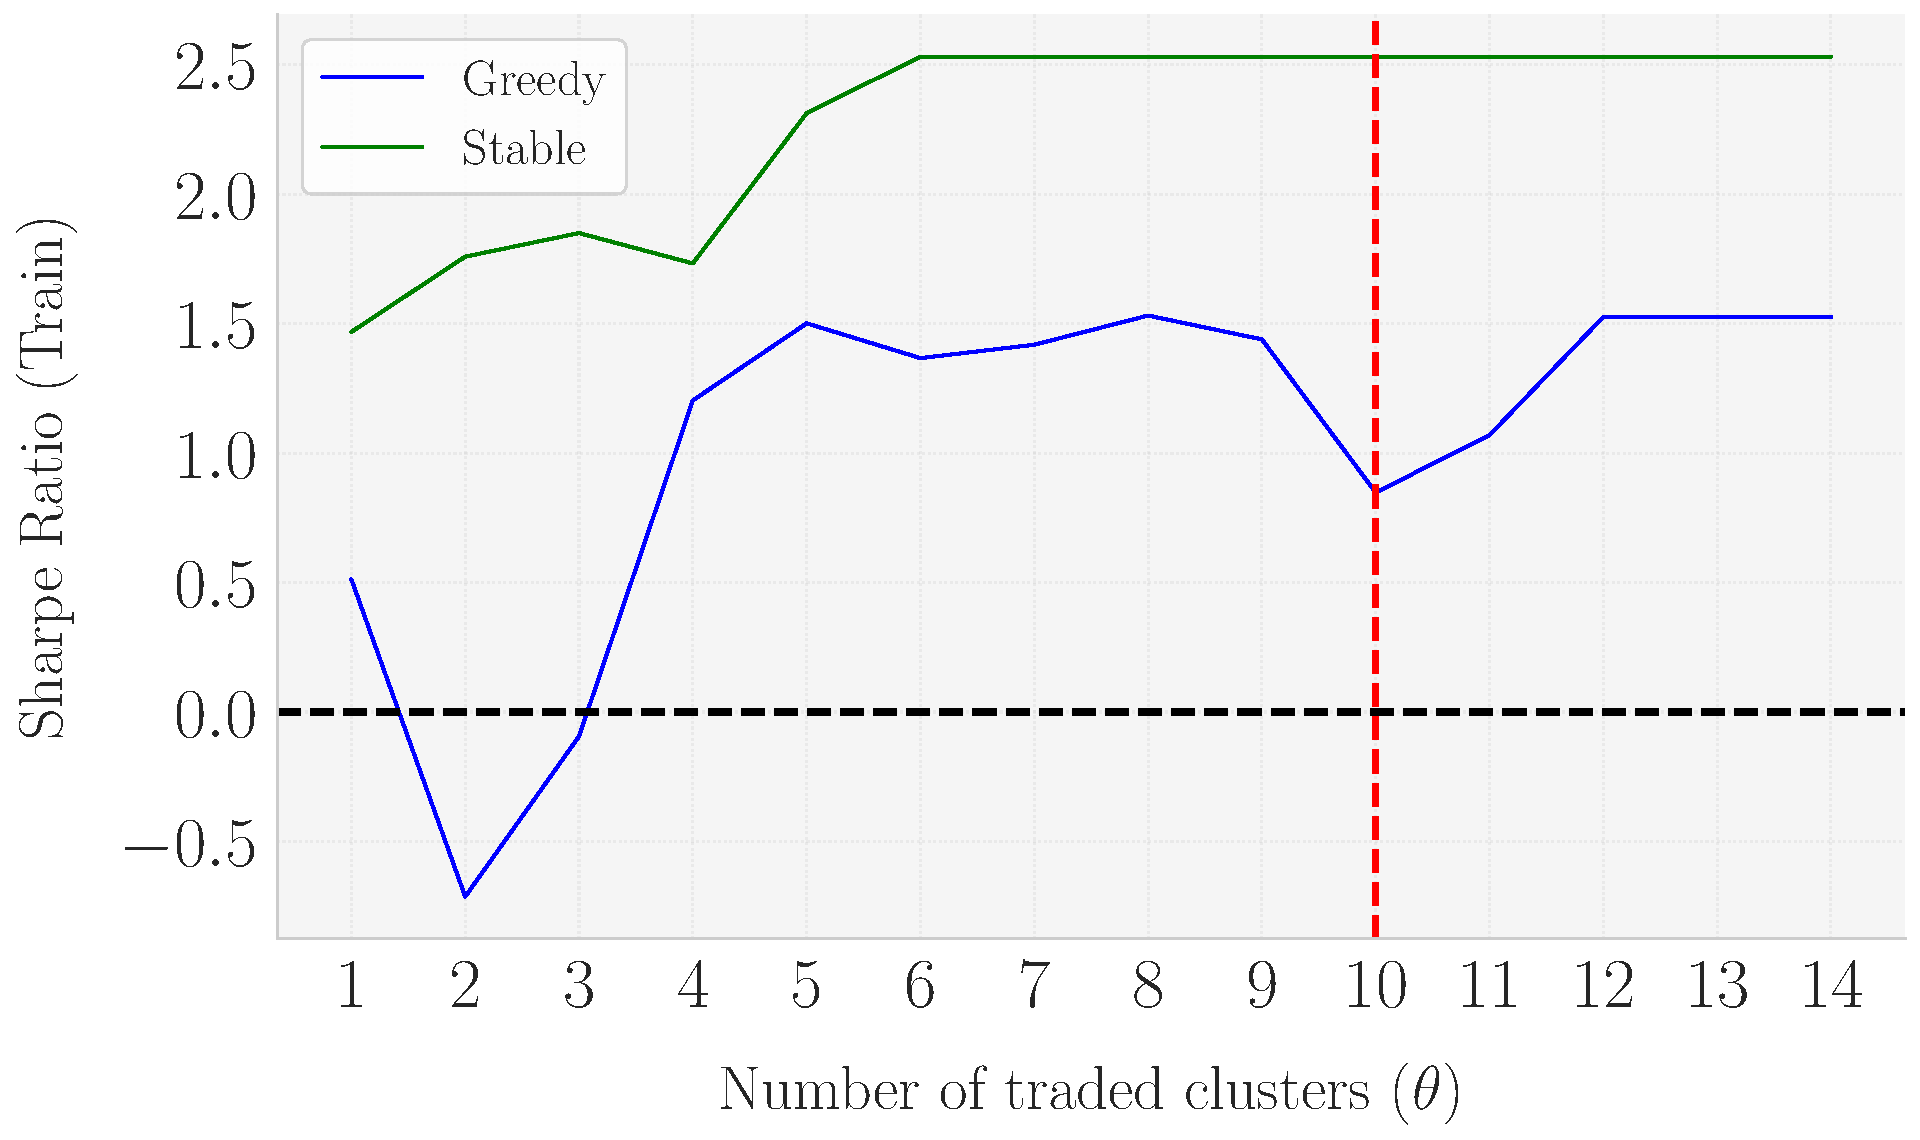
\includegraphics[width=\textwidth]{/Users/jesusvillotamiranda/Library/CloudStorage/OneDrive-UniversidaddeLaRioja/CEMFI/__MSc__/__Second_year__/6th_Term/MasterThesis/__Output/LLAMA_RobustnessCheck_SR_Train_Set_vs_Theta_[Change_theta].pdf}
    \caption{Plot of $SR^{\mathcal P^{tr}}(\theta)$ over a grid of $\theta$}
    \label{fig:LLM_hyp_3}
  \end{subfigure}
  \hspace{0.05\textwidth} % Add horizontal space between the subfigures
  \begin{subfigure}[b]{0.46\textwidth}
    \centering
    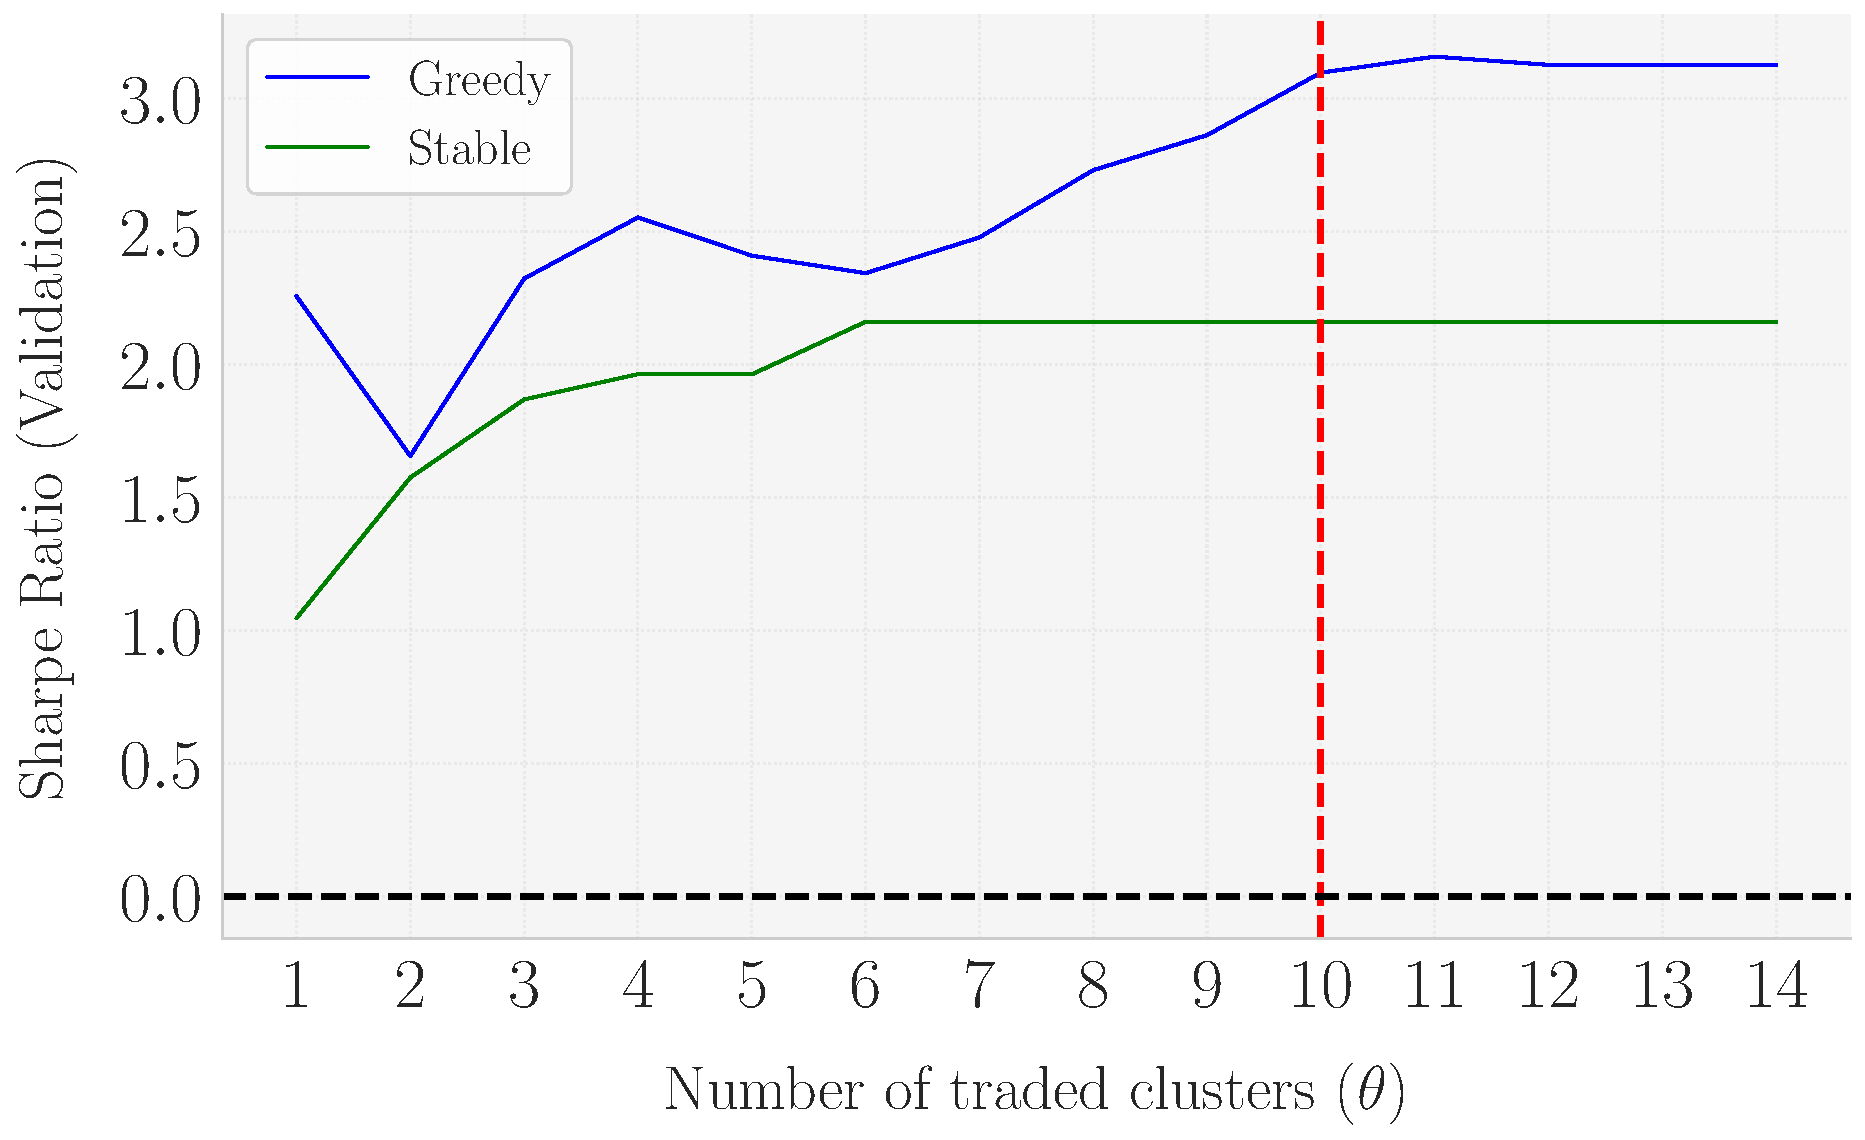
\includegraphics[width=\textwidth]{/Users/jesusvillotamiranda/Library/CloudStorage/OneDrive-UniversidaddeLaRioja/CEMFI/__MSc__/__Second_year__/6th_Term/MasterThesis/__Output/LLAMA_RobustnessCheck_SR_Validation_Set_vs_Theta_[Change_theta].pdf}
    \caption{Plot of $SR^{\mathcal P^{val}}(\theta)$ over a grid of $\theta$}
    \label{fig:LLM_hyp_4}
  \end{subfigure}
\mx
\subcaption*{\textit{Note: This figure illustrates the Sharpe Ratios ($SR$) as a function of $\theta$, the upper bound on the number of traded clusters, for the LLM clustering method in the training (Panel a) and validation (Panel b) splits. In Panel (a), the Sharpe Ratios for the training set indicate a temporary dip at $\theta=10$ for the Greedy algorithm, yet this value still provides a relatively stable outcome. In contrast, Panel (b) shows that $\theta=10$ leads to a noticeable increase in Sharpe Ratios for the validation set, particularly benefiting the Greedy algorithm. The choice of $\theta = \integer{0.5k} = 10$ strikes a balance, confirming it as an effective hyperparameter selection for achieving stability in both the training and validation splits with LLM clustering.}}
\label{fig:LLM_hyperparameter_justification_theta}
\end{figure}
%----------------------------------------------------


%%%%%%%%%%%%%%%%%%%%%%%%%%%%%%%%%%%%%%%%%%%%%%%%%%%%%

\newpage
%%%%%%%%%%%%%%%%%%%%%%%%%%%%%%%%%%%%%%%%%%%%%%%%%%%%%
\subsection{Optimal Cluster Selection Algorithms}
%%%%%%%%%%%%%%%%%%%%%%%%%%%%%%%%%%%%%%%%%%%%%%%%%%%%%
%----------------------------------------------------
\begin{algorithm}
\caption{
\textsc{Greedy Selection} 
~|~
{{Top average Sharpe Ratio in Validation Set}}
}
%%%%%%%%%%%%%%%%%%%%%%%%%%%%%%%%%%%%%%%%%%%%%%%%%%%%%
\label{alg:greedy_selection}
%%%%%%%%%%%%%%%%%%%%%%%%%%%%%%%%%%%%%%%%%%%%%%%%%%%%%
\begin{algorithmic}[1]
\mx 
\State \textbf{Input:} Set of clusters $\mathcal{G} = \{1, 2, \ldots, k^*\}$, Sharpe Ratios in the validation sample $\{SR_L^{(i,j)}\}_{(i,j)\in \mathcal B^{val}}$, maximum number of traded clusters $\theta\in\mathbb{N}$ (usually, $\theta\propto k^*)$

\mx 
\State \textbf{Output:} Set of long-traded clusters $\mathcal{G}_{\theta}^{+}$ and set of short-traded clusters $\mathcal{G}_{\theta}^{-}$
%----------------------------------------------------
%\Statex
\vspace{0.4cm}
\Statex \underline{\textit{Step \#1: Compute Cluster Average Sharpe Ratios in Validation Set}}
\For{each $g \in \mathcal{G}$}
    \State Compute average Sharpe Ratio ~
$
\overline{S R}_g^{val} \leftarrow \frac{1}{|\mathcal{B}_g^{val} |} \sum_{(i,j) \in \mathcal{B}_g^{val}} S R_{{{L}}}^{(i,j)}
$
\EndFor
%----------------------------------------------------
%\Statex
\vspace{0.4cm}
\Statex \underline{\textit{Step \#2: Identify Positive and Negative Sharpe Ratio Clusters}}
\State Define $\mathcal{G}_{SR^+}^{val} \leftarrow \{ g \in \mathcal{G} \mid \overline{SR}_g^{val} > 0 \}$
\State Define $\mathcal{G}_{SR^-}^{val} \leftarrow \{ g \in \mathcal{G} \mid \overline{SR}_g^{val} < 0 \}$
%----------------------------------------------------
\vspace{0.4cm}
\Statex \underline{\textit{Step \#3: Rank Clusters by Average Sharpe Ratio in the Validation Set}}
\For{each $g \in \mathcal{G}$}
	\State Rank the average Sharpe Ratio~~
$
\mathfrak{R}_g^{val} \leftarrow  \sum_{h \in \mathcal{G}} 
\mathbf{1}\1{
\overline{S R}_h^{val} \geq \overline{S R}_g^{val} 
}
$
\EndFor
%\State Sort clusters in descending order of $\overline{SR}_g^{val}$
%%\State
%$$\overline{SR}_{\varkappa_1}^{val} \geq \overline{SR}_{\varkappa_2}^{val} \geq \ldots \geq \overline{SR}_{\varkappa_{k^*}}^{val}$$
%----------------------------------------------------
%\Statex
\vspace{0.4cm}
\Statex \underline{\textit{Step \#4: Select Top $\theta$ Clusters}}
\State Define $\theta^+ \leftarrow \min(\theta, |\mathcal{G}_{SR^+}^{val}|)$
;~~
$\mathcal{G}_{\theta}^{+} \leftarrow \{ g\in\G \mid 1 \leq \mathfrak{R}_g^{val} \leq \theta^+ \}$
%\State 

\State Define $\theta^- \leftarrow \min(\theta, |\mathcal{G}_{SR^-}^{val}|)$
;~~
%\State 
 $\mathcal{G}_{\theta}^{-} \leftarrow \{ g \in\G \mid k^* - \theta^- < \mathfrak{R}_g^{val} \leq k^* \}$
%----------------------------------------------------
%\Statex
\vspace{0.5cm}
\State \textbf{Return} Long-traded clusters $\mathcal{G}_{\theta}^{+}$, Short-traded clusters $\mathcal{G}_{\theta}^{-}$

\end{algorithmic}
\end{algorithm}


%
%\begin{algorithm}[H]
%\caption{Greedy Selection of Clusters Based on Average Sharpe Ratio}
%%%%%%%%%%%%%%%%%%%%%%%%%%%%%%%%%%%%%%%%%%%%%%%%%%%%%%
%\label{alg:greedy_selection}
%%%%%%%%%%%%%%%%%%%%%%%%%%%%%%%%%%%%%%%%%%%%%%%%%%%%%%
%\begin{algorithmic}[1]
%\State \textbf{Input:} Set of clusters $\mathcal{G} = \{1, 2, \ldots, k^*\}$, Sharpe Ratios in the validation sample $\{SR_L^{(i,j)}\}_{(i,j)\in \mathcal{B}^{val}}$, maximum number of traded clusters $\theta \in \mathbb{N}$ (usually, $\theta \propto k^*$)
%\State \textbf{Output:} Set of long-traded clusters $\mathcal{G}_{\theta}^{+}$ and set of short-traded clusters $\mathcal{G}_{\theta}^{-}$
%
%\Statex
%\Statex \underline{\textit{Step \#1: Compute Cluster Average Sharpe Ratios in Validation Set}}
%\For{each $g \in \mathcal{G}$}
%    \State Compute average Sharpe Ratio ~
%    \[
%    \overline{SR}_g^{val} \leftarrow \frac{1}{|\mathcal{B}_g^{val} |} \sum_{(i,j) \in \mathcal{B}_g^{val}} SR_{L}^{(i,j)}
%    \]
%\EndFor
%
%\Statex
%\Statex \underline{\textit{Step \#2: Identify Positive and Negative Sharpe Ratio Clusters}}
%\State Define $\mathcal{G}_{SR^+}^{val} \leftarrow \{ g \in \mathcal{G} \mid \overline{SR}_g^{val} > 0 \}$
%\State Define $\mathcal{G}_{SR^-}^{val} \leftarrow \{ g \in \mathcal{G} \mid \overline{SR}_g^{val} < 0 \}$
%
%\Statex
%\Statex \underline{\textit{Step \#3: Rank Clusters by Average Sharpe Ratio}}
%\State Sort clusters in descending order of $\overline{SR}_g^{val}$
%%\State
%\[
%\overline{SR}_{\varkappa_1}^{val} \geq \overline{SR}_{\varkappa_2}^{val} \geq \ldots \geq \overline{SR}_{\varkappa_{k^*}}^{val}
%\]
%
%\Statex
%\Statex \underline{\textit{Step \#4: Select Top $\theta$ Clusters}}
%\State Define $\theta^+ \leftarrow \min(\theta, |\mathcal{G}_{SR^+}^{val}|)$
%\State Define $\theta^- \leftarrow \min(\theta, |\mathcal{G}_{SR^-}^{val}|)$
%
%\State Define $\mathcal{G}_{\theta}^{+} \leftarrow \{ \varkappa_{\ell} \in \mathcal{G} \mid 1 \leq \ell \leq \theta^+ \}$
%\State Define $\mathcal{G}_{\theta}^{-} \leftarrow \{ \varkappa_{\ell} \in \mathcal{G} \mid k^* - \theta^- < \ell \leq k^* \}$
%
%\Statex
%\State \textbf{Return} Long-traded clusters $\mathcal{G}_{\theta}^{+}$, Short-traded clusters $\mathcal{G}_{\theta}^{-}$
%
%\end{algorithmic}
%\end{algorithm}

%----------------------------------------------------


%----------------------------------------------------
\begin{algorithm}[H]
\caption{
\textsc{Rank Stability}
~ |~
{{Minimal Rank Difference between Train \& Validation Sets}
}}
%%%%%%%%%%%%%%%%%%%%%%%%%%%%%%%%%%%%%%%%%%%%%%%%%%%%%
\label{alg:rank_stability}
%%%%%%%%%%%%%%%%%%%%%%%%%%%%%%%%%%%%%%%%%%%%%%%%%%%%%
\begin{algorithmic}[1]
\mx 
\State \textbf{Input:} Set of clusters $\mathcal{G} = \{1, 2, \ldots, k^*\}$, Sharpe Ratios in the training and validation sample $\{SR_L^{(i,j)}\}_{(i,j)\in \mathcal B^{tr}}$ and $\{SR_L^{(i,j)}\}_{(i,j)\in \mathcal B^{val}}$, maximum number of traded clusters $\theta$
\mx 
\State \textbf{Output:} Set of long-traded clusters $\mathcal{G}_{\theta}^{+}$ and set of short-traded clusters $\mathcal{G}_{\theta}^{-}$
%----------------------------------------------------
%\Statex
\mx
\Statex \underline{\textit{Step \#1: Compute Cluster Average Sharpe Ratios in Training \& Validation Set}}
\For{each $g \in \mathcal{G}$}
    \State Compute average Sharpe Ratio in $\mathcal B^{tr}:$ ~~
$
\overline{S R}_g^{tr} \leftarrow \frac{1}{|\mathcal{B}_g^{tr} |} \sum_{(i,j) \in \mathcal{B}_g^{tr}} S R_{{{L}}}^{(i,j)}
$
    \State Compute average Sharpe Ratio in $\mathcal B^{val}:$ ~
$
\overline{S R}_g^{val} \leftarrow \frac{1}{|\mathcal{B}_g^{val} |} \sum_{(i,j) \in \mathcal{B}_g^{val}} S R_{{{L}}}^{(i,j)}
$
\EndFor
%----------------------------------------------------
%\Statex
\mx
\Statex \underline{\textit{Step \#2: Rank Clusters}}
%\State \# \textit{Step 1: Rank Clusters}
\For{each $g \in \mathcal{G}$}
    \State Rank the average Sharpe Ratios in $\mathcal B^{tr}:$ ~~
%$\{\overline{S R}_g^{tr}\}_{g\in\G}$ 
$
\mathfrak{R}_g^{tr} \leftarrow  \sum_{h \in \mathcal{G}} 
\mathbf{1}\1{
\overline{S R}_h^{t r} \geq \overline{S R}_g^{t r} 
}
$
    \State Rank the average Sharpe Ratios in $\mathcal B^{val}:$ ~
%$\{\overline{S R}_g^{tr}\}_{g\in\G}$ 
$
\mathfrak{R}_g^{val} \leftarrow  \sum_{h \in \mathcal{G}} 
\mathbf{1}\1{
\overline{S R}_h^{val} \geq \overline{S R}_g^{val} 
}
$
\EndFor
%----------------------------------------------------
%\Statex
\mx
\Statex \underline{\textit{Step \#3: Calculate Rank Differences}}
\For{each $g \in \mathcal{G}$}
    \State Calculate rank difference $\delta_g \leftarrow | \mathfrak R_g^{tr} - \mathfrak R_g^{val} |$
\EndFor
%----------------------------------------------------
%\Statex
\mx
\Statex \underline{\textit{Step \#4: Select Top $\theta$ Clusters with Smallest Rank Differences}}
\For{each $g \in \mathcal{G}$}
\State Rank the rank difference $:~~ \mathfrak{R}(\delta_g) \leftarrow \sum_{h\in\G} \mbf{1} \1{ \delta_g \geq  \delta_h }$
\EndFor
\State Select top $2\theta$ clusters with smallest $\delta_g$: 
$
~~
\mathcal{G}_{\theta} = 
\3{
g\in\G \c 1 \leq \mathfrak{R}(\delta_g) \leq 2\theta 
}
~
$
%----------------------------------------------------
%\Statex
\mx
\Statex \underline{\# \textit{Step 5: Determine Long and Short Positions}}
\State Define $\mathcal{G}_{\theta}^{+} = \{g \in \mathcal{G}_{\theta} \mid \overline{SR}_g^{tr} > 0 \text{ and } \overline{SR}_g^{val} > 0\}$
\State Define $\mathcal{G}_{\theta}^{-} = \{g \in \mathcal{G}_{\theta} \mid \overline{SR}_g^{tr} < 0 \text{ and } \overline{SR}_g^{val} < 0\}$
%----------------------------------------------------
%\Statex
\mx
\State \textbf{Return} Long-traded clusters $\mathcal{G}_{\theta}^{+}$, Short-traded clusters $\mathcal{G}_{\theta}^{-}$

\end{algorithmic}
\end{algorithm}


%----------------------------------------------------




%%%%%%%%%%%%%%%%%%%%%%%%%%%%%%%%%%%%%%%%%%%%%%%%%%%%%
\subsection{Sample of articles for each cluster}
%%%%%%%%%%%%%%%%%%%%%%%%%%%%%%%%%%%%%%%%%%%%%%%%%%%%%
\setcounter{table}{0}
\renewcommand{\thetable}{A\arabic{table}} % To ensure the tables in the appendix are numbered as A1, A2, etc.

%%----------------------------------------------------
%%%%%%%%%%%%%%%%%%%%%%%%%%%%%%%%%%%%%%%%%%%%%%%%%%%%%
%%%%%%%%%%%%%% 		ENGLISH 		%%%%%%%%%%%%%%%%%
%%%%%%%%%%%%%%%%%%%%%%%%%%%%%%%%%%%%%%%%%%%%%%%%%%%%%
%%%%%%%%%%%%%%%%%%%%%%%%%%%%%%%%%%%%%%%%%%%%%%%%%%%%%

\begin{landscape}
\renewcommand{\arraystretch}{1}

%\scriptsize
{\fontsize{9}{9}\selectfont % Set custom font size between \scriptsize and \tiny

%----------------------------------------------------
\begin{longtable}{|c|L{8cm}|L{14cm}|}
\caption{KMeans clustering. Proposed name for the clusters and sample of 3 articles for each cluster.} % Caption for the longtable
\label{tab:KMeans_Articles_3_English} \\
\hline 
\rowcolor{lightgray}
\# & \multicolumn{1}{c|}{Title} & \multicolumn{1}{c|}{Articles} \\
\hline \hline 
0 
& 
Miscellaneous (Colonial, Acciona, Amadeus, Grifols, Endesa, IAG, Bankinter...)
& 
\textbullet~Colonial forecasts rental income of EUR338m in 2020

\textbullet~Acciona's asset sales will allow it to grow in renewables

\textbullet~Sabadell recommends selling Amadeus shares due to worse sales forecast.
\\ \hline 
1
& 
Quarterly \& Semi-Annual Earnings Reports
& 
\textbullet~Enag�s 1H net profit falls 9.8\% due to lower income and extraordinary items.

\textbullet~Iberdrola: Net profit of EUR1.025m in Q1

\textbullet~Santander almost quintuples Q1 profit due to absence of Covid provisions.
\\ \hline 
2
& 
BBVA \& Sabadell: Financial Performance \& Strategic Movements
& 
\textbullet~Interest rate hike in Turkey favors BBVA's net interest margin

\textbullet~Sabadell reorganizes business in Spain following the arrival of the new CEO.

\textbullet~Fitch downgrades Banco Sabadell's rating one notch to low grade.
\\ \hline 
3
& 
Telef�nica \& Cellnex: Telecommunications Tower Sales \& Market Dynamics
& 
\textbullet~Telef�nica shares soar after selling towers of its subsidiary in Europe and Latin America.

\textbullet~Telef�nica hires Goldman Sachs to sell its British tower business

\textbullet~Dutch Competition Authority authorizes Cellnex to integrate 3,150 Deutsche Telekom towers.
\\ \hline 
4
& 
CaixaBank: Mergers and Strategic Moves in the Banking Sector
& 
\textbullet~CaixaBank and Bankia approve their merger project

\textbullet~CaixaBank closes its first issuance of green bonds in pounds for 500 million

\textbullet~CaixaBank-Bankia merger could generate EUR500m in savings
\\ \hline 
5
& 
Telef�nica, Indra, \& M�sM�vil: Regulatory and Strategic Moves in Telecom
& 
\textbullet~Indra to partner with Telef�nica in the deployment of fiber optics in Germany.

\textbullet~Telef�nica launches a buyback offer for its hybrid bonds of EUR1.000m.

\textbullet~EU refers Liberty Global and Telef�nica agreement to UK regulator
\\ \hline 
6
& 
Siemens Gamesa: Supply Agreements, Profitability Targets in Renewable Energy
& 
\textbullet~Siemens Gamesa will supply turbines to Elawan's 150 MW wind farm in Spain.

\textbullet~Siemens Gamesa lowers its profitability target for 2021.

\textbullet~Siemens Gamesa will supply 160 MW for the largest wind farm in the Philippines.
\\ \hline 
7
& 
Cellnex: Strategic Acquisitions and Financial Moves in Telecom Infrastructure
& 
\textbullet~Cellnex launches a EUR1.850m debt issue

\textbullet~Cellnex agrees to buy 10,500 telecommunications towers in France for EUR5.200m

\textbullet~Benetton family sells 2.5\% of Cellnex to Singapore sovereign fund
\\ \hline 
8
& 
Acciona, Endesa, Enag�s \& Naturgy: Strategic Moves \& Regulatory Developments in the Energy Sector
& 
\textbullet~Naturgy and Enag�s study project to produce green hydrogen in Asturias

\textbullet~Break of ties between Algeria and Morocco may damage gas flow to Spain

\textbullet~Acciona: Energy business IPO on track for 1H
\\ \hline 
9
& 
Repsol: Strategic Moves and Challenges in the Energy Sector
& 
\textbullet~Repsol to produce green hydrogen at Petronor refinery in 2022

\textbullet~Repsol and Talgo to jointly promote the creation of renewable hydrogen trains

\textbullet~Repsol gains access to a portfolio of renewable assets in Chile through a joint venture
\\ \hline 
10
& 
Ferrovial, Acciona: Strategic Expansions and Financial Maneuvers in Infrastructure
& 
\textbullet~Ferrovial closes the sale of Broadspectrum to Ventia for EUR291m

\textbullet~Acciona awarded the construction of 2 roads in Poland for EUR642m

\textbullet~Renfe awards on-board services contract to Ferrovial for EUR272m
\\ \hline 
11
& 
Solaria: Strategic Moves and Market Challenges in Renewable Energy
& 
\textbullet~Solaria invests EUR220m in Europe's largest photovoltaic park.

\textbullet~Solaria will supply energy to Shell and Axpo with Europe's largest photovoltaic plant

\textbullet~Goldman Sachs downgrades Solaria recommendation after stock rise.
\\ \hline 
12
& 
Iberdrola: Strategic Collaborations and Renewable Energy Developments
& 
\textbullet~Iberdrola will build a self-consumption plant for Lactalis factory in Spain.

\textbullet~Iberdrola and Mapfre launch a renewable energy co-investment vehicle in Spain.

\textbullet~Iberdrola partners with Mitsubishi to decarbonize the industry.
\\ \hline 
13
& 
IAG: Financial Performance
& 
\textbullet~IAG Q3 results worse than expected

\textbullet~IAG burns cash faster than anticipated

\textbullet~IAG stock may be pricing in a second capital increase
\\ \hline 
14
& 
Santander \& CaixaBank: Financial Moves and Sustainability Initiatives 
& 
\textbullet~CaixaBank mobilizes EUR12.000m in sustainable financing in the first 9 months of 2020.

\textbullet~EIB and Banco Santander will inject EUR587m into Portuguese SMEs.

\textbullet~Banco Santander, leader in renewable project financing in 2020.
\\ \hline 
15
& 
ACS \& Acciona: Strategic Movements and Infrastructure Projects
& 
\textbullet~ACS and Acciona win contracts for new Australian airport worth EUR164m.

\textbullet~Acciona awarded 3 contracts to operate wastewater treatment plants in Sardinia for EUR210m.

\textbullet~ACS expects net profit to grow by around 30\% in 2021
\\ \hline 
16
& 
Telef�nica: Financial Performance and Strategic Moves
& 
\textbullet~Reduction in Telef�nica's debt will improve analysts' perception

\textbullet~Telef�nica's profit more than doubles in Q1 due to lower financial expenses.

\textbullet~Telef�nica, Am�rica M�vil and TIM buy the mobile network of Brazil's Oi.
\\ \hline 
17
& 
Meli� and Spanish Tourism Sector: Challenges Amidst the Pandemic
& 
\textbullet~Meli�: Spanish hotel sector faces another uncertain summer with cautious optimism.

\textbullet~Meli� claims EUR116m from the Spanish government for pandemic-related damages.

\textbullet~Meli�: Local Covid-19 lockdowns will continue to affect Meli�.
\\ \hline 
18
& 
Takeover Bids for Naturgy and M�sM�vil
& 
\textbullet~Australian fund IFM launches EUR5.000m bid for 22.69\% of Naturgy.

\textbullet~Polygon fund asks CNMV to review and alter the bid for M�sM�vil.

\textbullet~IFM accepts Spanish government conditions in partial bid for Naturgy.
\\ \hline 
19
& 
Naturgy: Financial Performance
& 
\textbullet~Naturgy presents "weak" 2020 results

\textbullet~Naturgy may revise its strategic plan upwards due to gas prices.

\textbullet~Bank of America sees upside potential for Naturgy based on fundamentals.
\\ \hline 
20
& 
PharmaMar, Grifols: Regulatory Approvals and Market Moves in the Pharmaceutical Sector
& 
\textbullet~EU court annuls European Commission's refusal to market PharmaMar drug.

\textbullet~Grifols starts issuing EUR2.000m bonds to buy Biotest.

\textbullet~PharmaMar announces approval of lurbinectedin for lung cancer in Australia.
\\ \hline 
21
& 
Repsol: Financial Performance
& 
\textbullet~Repsol: Net loss of EUR3.289m in 2020.

\textbullet~Repsol reports a loss of EUR711m in Q4 due to exploration and production provisions

\textbullet~Repsol posts a loss of EUR94m in Q3 due to provisions and lower refining margins.
\\ \hline 
22
& 
Aena: Financial Performance
& 
\textbullet~JPMorgan raises Aena's target price to EUR155 from EUR135.

\textbullet~Aena risks a revenue cut of up to EUR2.000m due to rents.

\textbullet~Aena loses EUR170.7m in 1H as passenger traffic plummets due to the pandemic.
\\ \hline 
23
& 
Enag�s, Endesa, Iberdrola, Red El�ctrica: Regulatory and Market Challenges in the Energy Sector
& 
\textbullet~Spanish electric utilities will remain under pressure in the stock market 

\textbullet~Spanish government measures are bad news for the electric sector.

\textbullet~Spain's electricity price closes February with a 52\% drop vs January
\\ \hline 
24
& 
BBVA, CaixaBank, Banco Sabadell: Layoffs and Restructuring
& 
\textbullet~CaixaBank proposes to unions a redundancy plan affecting 8,291 employees.

\textbullet~Banco Santander closes its redundancy plan with 3,572 voluntary exits and 19 dismissals 

\textbullet~Sabadell prepares an adjustment plan affecting 2,000 employees
\\ \hline 
25
& 
Inditex, Acerinox: Market Performance and Strategic Developments in the Post-Covid Context
& 
\textbullet~Inditex reopens 94\% of its stores worldwide after Covid-19 pandemic.

\textbullet~Sale of Nippon Steel in Acerinox is negative, but expected.

\textbullet~Inditex stock already prices in a strong business recovery.
\\ \hline 
\end{longtable}
%----------------------------------------------------
}

\end{landscape}


%%%%%%%%%%%%%%%%%%%%%%%%%%%%%%%%%%%%%%%%%%%%%%%%%%%%%%
%%%%%%%%%%%%%%%%%%%%%%%%%%%%%%%%%%%%%%%%%%%%%%%%%%%%%%
%%%%%%%%%%%%%%% 		ENGLISH 		%%%%%%%%%%%%%%%%%
%%%%%%%%%%%%%%%%%%%%%%%%%%%%%%%%%%%%%%%%%%%%%%%%%%%%%%
%%%%%%%%%%%%%%%%%%%%%%%%%%%%%%%%%%%%%%%%%%%%%%%%%%%%%%
%
%\begin{landscape}
%\renewcommand{\arraystretch}{1}
%
%
%%\scriptsize
%{\fontsize{9}{9}\selectfont % Set custom font size between \scriptsize and \tiny
%
%
%
%%----------------------------------------------------
%\begin{longtable}{|c|L{8cm}|L{14cm}|}
%\caption{KMeans clustering. Proposed name for the clusters and sample of 3 articles for each cluster.} \\ % Caption for the longtable
%\hline 
%\rowcolor{lightgray}
%\# & \multicolumn{1}{c|}{Title} & \multicolumn{1}{c|}{Articles} \\
%\hline \hline 
%0 
%& 
%Miscellaneous (Colonial, Acciona, Amadeus, Grifols, Endesa, IAG, Bankinter...)
%& 
%\textbullet~Colonial forecasts rental income of EUR338m in 2020
%
%\textbullet~Acciona's asset sales will allow it to grow in renewables
%
%\textbullet~Sabadell recommends selling Amadeus shares due to worse sales forecast.
%\\ \hline 
%1
%& 
%Quarterly \& Semi-Annual Earnings Reports
%& 
%\textbullet~Enag�s 1H net profit falls 9.8\% due to lower income and extraordinary items.
%
%\textbullet~Iberdrola: Net profit of EUR1.025m in Q1
%
%\textbullet~Santander almost quintuples Q1 profit due to absence of Covid provisions.
%\\ \hline 
%2
%& 
%BBVA \& Sabadell: Financial Performance \& Strategic Movements
%& 
%\textbullet~Interest rate hike in Turkey favors BBVA's net interest margin
%
%\textbullet~Sabadell reorganizes business in Spain following the arrival of the new CEO.
%
%\textbullet~Fitch downgrades Banco Sabadell's rating one notch to low grade.
%\\ \hline 
%3
%& 
%Telef�nica \& Cellnex: Telecommunications Tower Sales \& Market Dynamics
%& 
%\textbullet~Telef�nica shares soar after selling towers of its subsidiary in Europe and Latin America.
%
%\textbullet~Telef�nica hires Goldman Sachs to sell its British tower business
%
%\textbullet~Dutch Competition Authority authorizes Cellnex to integrate 3,150 Deutsche Telekom towers.
%\\ \hline 
%4
%& 
%CaixaBank: Mergers and Strategic Moves in the Banking Sector
%& 
%\textbullet~CaixaBank and Bankia approve their merger project
%
%\textbullet~CaixaBank closes its first issuance of green bonds in pounds for 500 million
%
%\textbullet~CaixaBank-Bankia merger could generate EUR500m in savings
%\\ \hline 
%5
%& 
%Telef�nica, Indra, \& M�sM�vil: Regulatory and Strategic Moves in Telecom
%& 
%\textbullet~Indra to partner with Telef�nica in the deployment of fiber optics in Germany.
%
%\textbullet~Telef�nica launches a buyback offer for its hybrid bonds of EUR1.000m.
%
%\textbullet~EU refers Liberty Global and Telef�nica agreement to UK regulator
%\\ \hline 
%6
%& 
%Siemens Gamesa: Supply Agreements, Profitability Targets in Renewable Energy
%& 
%\textbullet~Siemens Gamesa will supply turbines to Elawan's 150 MW wind farm in Spain.
%
%\textbullet~Siemens Gamesa lowers its profitability target for 2021.
%
%\textbullet~Siemens Gamesa will supply 160 MW for the largest wind farm in the Philippines.
%\\ \hline 
%7
%& 
%Cellnex: Strategic Acquisitions and Financial Moves in Telecom Infrastructure
%& 
%\textbullet~Cellnex launches a EUR1.850m debt issue
%
%\textbullet~Cellnex agrees to buy 10,500 telecommunications towers in France for EUR5.200m
%
%\textbullet~Benetton family sells 2.5\% of Cellnex to Singapore sovereign fund
%\\ \hline 
%8
%& 
%Acciona, Endesa, Enag�s \& Naturgy: Strategic Moves \& Regulatory Developments in the Energy Sector
%& 
%\textbullet~Naturgy and Enag�s study project to produce green hydrogen in Asturias
%
%\textbullet~Break of ties between Algeria and Morocco may damage gas flow to Spain
%
%\textbullet~Acciona: Energy business IPO on track for 1H
%\\ \hline 
%9
%& 
%Repsol: Strategic Moves and Challenges in the Energy Sector
%& 
%\textbullet~Repsol to produce green hydrogen at Petronor refinery in 2022
%
%\textbullet~Repsol and Talgo to jointly promote the creation of renewable hydrogen trains
%
%\textbullet~Repsol gains access to a portfolio of renewable assets in Chile through a joint venture
%\\ \hline 
%10
%& 
%Ferrovial, Acciona: Strategic Expansions and Financial Maneuvers in Infrastructure
%& 
%\textbullet~Ferrovial closes the sale of Broadspectrum to Ventia for EUR291m
%
%\textbullet~Acciona awarded the construction of 2 roads in Poland for EUR642m
%
%\textbullet~Renfe awards on-board services contract to Ferrovial for EUR272m
%\\ \hline 
%11
%& 
%Solaria: Strategic Moves and Market Challenges in Renewable Energy
%& 
%\textbullet~Solaria invests EUR220m in Europe's largest photovoltaic park.
%
%\textbullet~Solaria will supply energy to Shell and Axpo with Europe's largest photovoltaic plant
%
%\textbullet~Goldman Sachs downgrades Solaria recommendation after stock rise.
%\\ \hline 
%12
%& 
%Iberdrola: Strategic Collaborations and Renewable Energy Developments
%& 
%\textbullet~Iberdrola will build a self-consumption plant for Lactalis factory in Spain.
%
%\textbullet~Iberdrola and Mapfre launch a renewable energy co-investment vehicle in Spain.
%
%\textbullet~Iberdrola partners with Mitsubishi to decarbonize the industry.
%\\ \hline 
%13
%& 
%IAG: Financial Performance
%& 
%\textbullet~IAG Q3 results worse than expected
%
%\textbullet~IAG burns cash faster than anticipated
%
%\textbullet~IAG stock may be pricing in a second capital increase
%\\ \hline 
%14
%& 
%Santander \& CaixaBank: Financial Moves and Sustainability Initiatives 
%& 
%\textbullet~CaixaBank mobilizes EUR12.000m in sustainable financing in the first 9 months of 2020.
%
%\textbullet~EIB and Banco Santander will inject EUR587m into Portuguese SMEs.
%
%\textbullet~Banco Santander, leader in renewable project financing in 2020.
%\\ \hline 
%15
%& 
%ACS \& Acciona: Strategic Movements and Infrastructure Projects
%& 
%\textbullet~ACS and Acciona win contracts for new Australian airport worth EUR164m.
%
%\textbullet~Acciona awarded 3 contracts to operate wastewater treatment plants in Sardinia for EUR210m.
%
%\textbullet~ACS expects net profit to grow by around 30\% in 2021
%\\ \hline 
%16
%& 
%Telef�nica: Financial Performance and Strategic Moves
%& 
%\textbullet~Reduction in Telef�nica's debt will improve analysts' perception
%
%\textbullet~Telef�nica's profit more than doubles in Q1 due to lower financial expenses.
%
%\textbullet~Telef�nica, Am�rica M�vil and TIM buy the mobile network of Brazil's Oi.
%\\ \hline 
%17
%& 
%Meli� and Spanish Tourism Sector: Challenges Amidst the Pandemic
%& 
%\textbullet~Meli�: Spanish hotel sector faces another uncertain summer with cautious optimism.
%
%\textbullet~Meli� claims EUR116m from the Spanish government for pandemic-related damages.
%
%\textbullet~Meli�: Local Covid-19 lockdowns will continue to affect Meli�.
%\\ \hline 
%18
%& 
%Takeover Bids for Naturgy and M�sM�vil
%& 
%\textbullet~Australian fund IFM launches EUR5.000m bid for 22.69\% of Naturgy.
%
%\textbullet~Polygon fund asks CNMV to review and alter the bid for M�sM�vil.
%
%\textbullet~IFM accepts Spanish government conditions in partial bid for Naturgy.
%\\ \hline 
%19
%& 
%Naturgy: Financial Performance
%& 
%\textbullet~Naturgy presents "weak" 2020 results
%
%\textbullet~Naturgy may revise its strategic plan upwards due to gas prices.
%
%\textbullet~Bank of America sees upside potential for Naturgy based on fundamentals.
%\\ \hline 
%20
%& 
%PharmaMar, Grifols: Regulatory Approvals and Market Moves in the Pharmaceutical Sector
%& 
%\textbullet~EU court annuls European Commission's refusal to market PharmaMar drug.
%
%\textbullet~Grifols starts issuing EUR2.000m bonds to buy Biotest.
%
%\textbullet~PharmaMar announces approval of lurbinectedin for lung cancer in Australia.
%\\ \hline 
%21
%& 
%Repsol: Financial Performance
%& 
%\textbullet~Repsol: Net loss of EUR3.289m in 2020.
%
%\textbullet~Repsol reports a loss of EUR711m in Q4 due to exploration and production provisions
%
%\textbullet~Repsol posts a loss of EUR94m in Q3 due to provisions and lower refining margins.
%\\ \hline 
%22
%& 
%Aena: Financial Performance
%& 
%\textbullet~JPMorgan raises Aena's target price to EUR155 from EUR135.
%
%\textbullet~Aena risks a revenue cut of up to EUR2.000m due to rents.
%
%\textbullet~Aena loses EUR170.7m in 1H as passenger traffic plummets due to the pandemic.
%\\ \hline 
%23
%& 
%Enag�s, Endesa, Iberdrola, Red El�ctrica: Regulatory and Market Challenges in the Energy Sector
%& 
%\textbullet~Spanish electric utilities will remain under pressure in the stock market 
%
%\textbullet~Spanish government measures are bad news for the electric sector.
%
%\textbullet~Spain's electricity price closes February with a 52\% drop vs January
%\\ \hline 
%24
%& 
%BBVA, CaixaBank, Banco Sabadell: Layoffs and Restructuring
%& 
%\textbullet~CaixaBank proposes to unions a redundancy plan affecting 8,291 employees.
%
%\textbullet~Banco Santander closes its redundancy plan with 3,572 voluntary exits and 19 dismissals 
%
%\textbullet~Sabadell prepares an adjustment plan affecting 2,000 employees
%\\ \hline 
%25
%& 
%Inditex, Acerinox: Market Performance and Strategic Developments in the Post-Covid Context
%& 
%\textbullet~Inditex reopens 94\% of its stores worldwide after Covid-19 pandemic.
%
%\textbullet~Sale of Nippon Steel in Acerinox is negative, but expected.
%
%\textbullet~Inditex stock already prices in a strong business recovery.
%\\ \hline 
%\end{longtable}
%%----------------------------------------------------
%}
%
%\end{landscape}

%%----------------------------------------------------

%----------------------------------------------------
%%%%%%%%%%%%%%%%%%%%%%%%%%%%%%%%%%%%%%%%%%%%%%%%%%%%%
%%%%%%%%%%%%%%%%%%%%%%%%%%%%%%%%%%%%%%%%%%%%%%%%%%%%%
%%%%%%%%%%%%%% 3 ARTICLES PER CLUSTER %%%%%%%%%%%%%%%
%%%%%%%%%%%%%%%%%%%%%%%%%%%%%%%%%%%%%%%%%%%%%%%%%%%%%
%%%%%%%%%%%%%%%%%%%%% ENGLISH %%%%%%%%%%%%%%%%%%%%%%%
%%%%%%%%%%%%%%%%%%%%%%%%%%%%%%%%%%%%%%%%%%%%%%%%%%%%%
%%%%%%%%%%%%%%%%%%%%%%%%%%%%%%%%%%%%%%%%%%%%%%%%%%%%%

\begin{landscape}
\renewcommand{\arraystretch}{1}


%\scriptsize
{\fontsize{10}{10}\selectfont % Set custom font size between \scriptsize and \tiny


%----------------------------------------------------
\begin{longtable}{|c|L{8cm}|L{14cm}|}
\caption{LLM clustering. Sample of 3 articles for each cluster.} 
\label{tab:LLM_Articles_3_English} \\
\hline 
\rowcolor{lightgray}
\# & \multicolumn{1}{c|}{Title} & \multicolumn{1}{c|}{Articles} \\
\hline \hline 
0 
& 
Demand, Minor, Positive
& 
\textbullet~Meli�'s recovery will be fast, but it will not be completed until 2023

\textbullet~Tourism sector aid in Spain will have a limited impact on listed companies

\textbullet~Spanish airports will recover pre-pandemic traffic by the end of 2025
\\ \hline 
1
& 
Demand, Minor, Negative
& 
\textbullet~Tallgrass will contribute fewer dividends to Enag�s -JPMorgan Cazenove

\textbullet~Aena's stock decline is due to sector visibility -Sabadell

\textbullet~ObservaTUR believes Spain's economic situation will worsen and calls for more measures
\\ \hline 
2
& 
Demand, Major, Positive
& 
\textbullet~Solaria invests EUR220m in Europe's largest photovoltaic park

\textbullet~Acciona will build Sao Paulo metro line for EUR2.3 billion

\textbullet~Inditex returns to profit in H1 and continues to recover from the pandemic
\\ \hline 
3
& 
Demand, Major, Negative
& 
\textbullet~Passenger traffic at Aena airports falls 79.9\% year-on-year in September

\textbullet~UPDATE: Naturgy's net profit falls 45.6\% in 9m due to Covid-19 impact

\textbullet~Possible capital increase by IAG already priced in
\\ \hline 
4
& 
Supply, Minor, Positive
& 
\textbullet~Repsol returns to profit in Q2 due to crude price increase

\textbullet~Naturgy receives LNG supply contract for ships for 2 years in Spain

\textbullet~Acciona Energ�a starts up 238 MW photovoltaic complex in Chile
\\ \hline 
5
& 
Supply, Minor, Negative
& 
\textbullet~Enag�s operating results worse than expected -Bankinter

\textbullet~IFM rules out extending acceptance period for Naturgy takeover bid and changing conditions

\textbullet~Changes in Siemens Gamesa's onshore wind business will take time
\\ \hline 
6
& 
Supply, Major, Positive
& 
\textbullet~Capital Energy wins renewable auction in Spain

\textbullet~Repsol expects to start exploiting its huge gas reserve in Brazil in 2026

\textbullet~Repsol will invest EUR657m to expand its industrial complex in Sines, Portugal
\\ \hline 
7
& 
Supply, Major, Negative
& 
\textbullet~Iberdrola halts \$1.2 billion investment in Mexico

\textbullet~85\% of Acciona workers at Nissan agree to contract termination

\textbullet~CaixaBank reduces workforce adjustment by 500 employees to 7,791 -Source
\\ \hline 
8
& 
Financial, Minor, Positive
& 
\textbullet~Norwegian fund Norges Bank takes 1.14\% stake in Naturgy amid IFM takeover bid

\textbullet~Sabadell closes green bond issue for EUR500m -Source

\textbullet~CaixaBank-Bankia merger goals are credible -Deutsche Bank
\\ \hline 
9
& 
Financial, Minor, Negative
& 
\textbullet~UPDATE2: Bankia's profit falls 57.6\% in 2020 due to provisions for pandemic impact

\textbullet~Iberdrola bond spreads will not be affected by Gal�n's indictment for now

\textbullet~Court maintains precautionary suspension of rent payments to Aena
\\ \hline 
10
& 
Financial, Major, Positive
& 
\textbullet~UPDATE: Endesa's net profit soars in 2020 due to lower impairment charges

\textbullet~Telef�nica will reduce debt by EUR5bn after closing Virgin Media and O2 merger

\textbullet~Fluidra buys US company S.R. Smith for \$240m
\\ \hline 
11
& 
Financial, Major, Negative
& 
\textbullet~UPDATE3: Banco Santander reports EUR8.771bn loss in 2020 due to Covid charges

\textbullet~Bankinter downgrades Grifols recommendation to neutral from buy

\textbullet~BBVA reduces layoffs to 3,361 and proposes early retirement at 52 with 65\% salary
\\ \hline 
12
& 
Technology, Minor, Positive
& 
\textbullet~Siemens Gamesa to supply turbines for 298MW wind farm in the US

\textbullet~Repsol and Técnicas Reunidas team up to develop decarbonization technologies

\textbullet~European Commission funds Repsol and Enag�s renewable hydrogen project
\\ \hline 
13
& 
Technology, Minor, Negative
& 
\textbullet~Cellnex and REE apply for EU funds to develop rural mobile networks
\\ \hline 
14
& 
Technology, Major, Positive
& 
\textbullet~Telef�nica and Allianz partner to deploy fiber in Germany

\textbullet~Iberdrola partners with Cosmo to develop 600 MW of offshore wind in Japan

\textbullet~Telef�nica estimates 5G network will require over EUR6bn in Spain
\\ \hline 
15
& 
Technology, Major, Negative
& 
X
\\ \hline 
16
& 
Policy, Minor, Positive
& 
\textbullet~Enag�s promotes 34 hydrogen and 21 biomethane proposals to recovery funds

\textbullet~Iberdrola president sees need to reform taxation to make renewables competitive

\textbullet~New electricity tariff in Spain aims to change consumer habits -Experts
\\ \hline 
17
& 
Policy, Minor, Negative
& 
\textbullet~Spanish government measures hurt Iberdrola -IG

\textbullet~Spanish government plans law to reduce CO2 price impact on electricity bills -Source

\textbullet~Iberdrola CEO criticizes electricity reform in Spain for "unexpected charges"
\\ \hline 
18
& 
Policy, Major, Positive
& 
\textbullet~Endesa is Spain's future green leader, but trades at a discount

\textbullet~TCI fund supports ACS's interest in ASPI and will reject Italy's offer

\textbullet~Cellnex acquisition in France reassures investors -Berenberg
\\ \hline 
19
& 
Policy, Major, Negative
& 
\textbullet~Sabadell does not expect improvement in partial takeover bid price for Naturgy

\textbullet~Renta 4 downgrades Naturgy to underweight after government measures

\textbullet~Bankinter warns of uncertainties over Iberdrola stock
\\ \hline 
\end{longtable}
%----------------------------------------------------
}
\end{landscape}

%----------------------------------------------------




%%%%%%%%%%%%%%%%%%%%%%%%%%%%%%%%%%%%%%%%%%%%%%%%%%%%%
\subsection{Function Calling with LLaMA-3}
%%%%%%%%%%%%%%%%%%%%%%%%%%%%%%%%%%%%%%%%%%%%%%%%%%%%%
%----------------------------------------------------
\definecolor{lightgray}{gray}{0.6} % Define a light gray color

\begin{algorithm}[H]
\caption{Function Calling Workflow for LLaMA-3}
%%%%%%%%%%%%%%%%%%%%%%%%%%%%%%%%%%%%%%%%%%%%%%%%%%%%%
\label{alg:function_calling}
%%%%%%%%%%%%%%%%%%%%%%%%%%%%%%%%%%%%%%%%%%%%%%%%%%%%%
\begin{algorithmic}[1]
\Require $\D$: Dataset of news articles
\Ensure Structured JSON output for each article
\State Initialize LLaMA-3 model via GroqCloud API
\For{each article $i \in \D$} \Comment{\scalebox{0.9}{\textcolor{lightgray}{Iterate over each article in the dataset}}}
%    \State Set up system message with instructions for LLM
    \State \textbf{Message: System} \Comment{\scalebox{0.9}{\textcolor{lightgray}{Define the role and task for the LLM}}}
%        \Statex \hspace{1cm} You are a function calling LLM that analyzes business news in Spanish. For every article, 
%
%\hspace{0.3cm} identify the firms that are directly affected by the news and classify the shocks in type, 
%
%\hspace{0.3cm} magnitude and direction

		\begin{quote}
			\qquote{You are a function calling LLM that analyzes business news in Spanish. For every article, identify the firms that are directly affected by the news and classify the shocks in type, magnitude and direction}
		\end{quote}


%as follows:
%    \Statex \hspace{1cm} \textit{Type}: \{demand, supply, financial, policy, technology\}
%    \Statex \hspace{1cm} \textit{Magnitude}: \{minor, major\}
%    \Statex \hspace{1cm} \textit{Direction}: \{positive, negative\}
%    \State Prepare user prompt $P_i$ containing the text of article $i$ \Comment{\scalebox{0.9}{\textcolor{lightgray}{Input the article text}}
    \State \textbf{Message: User} \Comment{\scalebox{0.9}{\textcolor{lightgray}{User provides the article text as input}}}
    \Statex \hspace{1cm} Content: prompt $P_i$ containing the text of article $i$
%    \State Define tools, including the \texttt{news\_parser} function \Comment{\scalebox{0.9}{\textcolor{lightgray}{Specify the functions to be used}}}
    \State \textbf{Tool: news\_parser} \Comment{\scalebox{0.9}{\textcolor{lightgray}{Define the \texttt{news\_parser} function}}}
%    \Statex \hspace{1cm} Parameters: \{firms: array of objects\}
%    \Statex \hspace{1cm} \textit{Each object contains:}
%    
\begin{quote}
\begin{quote}
Parameters: \{\texttt{firms}: \bblue{\texttt{array}} of objects\}, where each object contains:
            \begin{itemize}
                \item \texttt{firm}: \hspace{2.1cm} \bblue{\texttt{string}} (\qquote{each one firm in \texttt{firms}})
                \item \texttt{ticker}: \hspace{1.7cm} \bblue{\texttt{string}} (\qquote{stock market ticker})
                \item \texttt{shock\_type}: \hspace{0.9cm} \bblue{\texttt{enum}} \{demand, supply, financial, policy, technology\}
                \item \texttt{shock\_magnitude}:  \hspace{0cm}\bblue{\texttt{enum}} \{minor, major\}
                \item \texttt{shock\_direction}: \hspace{0cm}\bblue{\texttt{enum}} \{positive, negative\}
            \end{itemize} 
\end{quote} 
\end{quote} 
 
     
%    \Statex \hspace{1cm} - \texttt{firm}: string (publicly listed Spanish firm)
%    \Statex \hspace{1cm} - \texttt{ticker}: string (e.g., TICKER.MC)
%    \Statex \hspace{1cm} - \texttt{shock\_type}: \{demand, supply, financial, policy, technology\}
%    \Statex \hspace{1cm} - \texttt{shock\_magnitude}: \{minor, major\}
%    \Statex \hspace{1cm} - \texttt{shock\_direction}: \{positive, negative\}
    \State Send initial messages and tools to LLaMA-3 \Comment{\scalebox{0.9}{\textcolor{lightgray}{Initiate interaction with the LLM}}}
    \State Retrieve response from LLaMA-3 \Comment{\scalebox{0.9}{\textcolor{lightgray}{Get the initial response from the LLM}}}
    \If{Function call is requested by LLaMA-3} \Comment{\scalebox{0.9}{\textcolor{lightgray}{Check if the LLM needs to call a function}}}
        \State Execute \texttt{news\_parser} function with provided arguments \Comment{\scalebox{0.9}{\textcolor{lightgray}{Run the function}}}
        \State Append function response to the conversation \Comment{\scalebox{0.9}{\textcolor{lightgray}{Include function output in the dialogue}}}
        \State Send updated messages to LLaMA-3 \Comment{\scalebox{0.9}{\textcolor{lightgray}{Continue the conversation with new information}}}
        \State Retrieve final response from LLaMA-3 \Comment{\scalebox{0.9}{\textcolor{lightgray}{Get the final output from the LLM}}}
    \EndIf
    \State Extract and store structured JSON output \Comment{\scalebox{0.9}{\textcolor{lightgray}{Save the processed data}}}
\EndFor
\end{algorithmic}
\end{algorithm}

%----------------------------------------------------


%%%%%%%%%%%%% BENCHMARK COMPARISON %%%%%%%%%%%%%%%%%%%
%----------------------------------------------------
\subsection{Why not using a different benchmark?}

In evaluating our novel Large Language Model (LLM) methodology for classifying news-implied firm-specific shocks, it is imperative to establish a robust and relevant benchmark. Our chosen benchmark involves transforming news articles into high-dimensional vector embeddings followed by clustering these embeddings using the KMeans algorithm. This section delineates the rationale behind selecting KMeans clustering of vector embeddings over other potential benchmarks such as sentiment analysis and topic modeling.

%%%%%%%%%%%%%%%%%%%%%%%%%%%%%%%%%%%%%%%%%%%%%%%%%%%%%
%%%%%%%%%%%%%%%%%%%%%%%%%%%%%%%%%%%%%%%%%%%%%%%%%%%%%
%%%%%%%%%%%%%%%%%%%%%%%%%%%%%%%%%%%%%%%%%%%%%%%%%%%%%
%%%%%%%%%%%%%%%%%%%%%%%%%%%%%%%%%%%%%%%%%%%%%%%%%%%%%

\subsubsection*{Why not Sentiment Analysis as a benchmark?}

Sentiment analysis is a widely recognized technique in natural language processing that aims to determine the emotional tone conveyed in a text, typically categorizing content as positive, negative, or neutral. While sentiment analysis provides a straightforward approach to gauging the general tone of news articles, it falls short in several critical aspects when juxtaposed with our objectives.

%\paragraph{Lack of Granularity}

First, sentiment analysis is not sufficiently granular. Our LLM methodology classifies news articles into 20 distinct categories of economic shocks while sentiment analysis classifies articles in a coarse manner, typically into positive, negative, or neutral categories, which is inadequate for benchmarking a detailed classification model. 

%\paragraph{Economic Irrelevance}

Second, sentiment analysis predominantly focuses on the linguistic and emotional aspects of the text, which do not necessarily correlate with the economic impact on firms. For instance, a neutral-toned article could describe a significant economic event, while a positive sentiment might not always translate to favorable economic outcomes. Consequently, the sentiment does not provide direct insights into the economic consequences, making it an economically irrelevant benchmark for our purposes.

%\paragraph{Sensitivity to Linguistic Nuances}

Third, sentiment analysis algorithms are often sensitive to linguistic subtleties, leading to inconsistent results across different languages and contexts. For example, sarcasm or idiomatic expressions can distort sentiment scores, undermining the reliability of sentiment analysis as a benchmark. 
This variability poses a challenge for standardization, especially in a multilingual context. For instance, the sentiment derived from analyzing the text in English may significantly differ from the sentiment in Spanish. 

%\paragraph{Lack of Robustness}

Fourth, sentiment analysis is not robust in the sense that different sentiment analysis tools yield divergent assessments of the same text. As shown below, we observe considerable differences in the identified sentiment when applying multiple sentiment analysis providers to a specific article. This lack of consistency undermines the reliability of sentiment analysis as a benchmark, making it unsuitable for our purposes.

\begin{quote}
\textit{
Sentiment analysis is highly sensitive to the specific tool
or model employed. Here, we demonstrate this by analyzing a piece of
business news using various popular sentiment analysis tools:
\texttt{TextBlob}, \texttt{text2data}, \texttt{VADER}, and
\texttt{FinBERT}. The methods vary significantly in both their approach
to sentiment determination and the output they provide, as illustrated
below.}%------------------- BEGIN FOOTNOTE -------------------------
\footnote{Note that applying Loughran-Macdonald is not recommended in for short texts as it yields sparse results. For example, in the example we are considering, it outputs a category distribution that only loads on \qquote{Strong Modal}, which is not a really useful analysis.
 
\texttt{
LM\_Scores = \{'Negative': 0, 'Positive': 0, 'Uncertainty': 0, 'Litigious': 0, 
'Strong\_Modal': 2, 'Weak\_Modal': 0, 'Constraining': 0, 'Complexity': 0\}}
}
\end{quote}
%--------------------- END FOOTNOTE -----------------------------

%%%%%%%%%%%%%%%%%%%%%%%%%%%%%%%%%%%%%%%%%%%%%%%%%%%%%

\begin{news}
    [A news article about Telef�nica and Cellnex | Sentiment: \texttt{TextBlob}]  
    [news:cellnex-article]                            
    {\green{Cellnex will face more competition in Europe} \resubp[dark_green]{\text{~\textnormal{\textbf{Score: 0.50}}~}}} 
    \bblue{Telef�nica's (TEF.MC) subsidiary, Telxius Telecom, has agreed to sell its telecommunications tower division in Europe and Latin America to American Tower (AMT), which will expand the latter's presence in Europe and increase competition for the Spanish wireless telecommunications group Cellnex Telecom (CLNX.MC), according to Equita Sim.}
    \resubp[blue]{\text{~\textnormal{\textbf{Score: 0.00}}~}}\bluegreen{The transaction "represents the entry of a new independent tower operator into the Spanish market and potentially more competition for future growth in the European market as well," says the brokerage firm.} \resubp[bluegreen]{\text{~\textnormal{\textbf{Score: 0.06}}~}} 


\vspace{0.5cm}
{\centering  
\textnormal{\textsc{Overall}} 
 \resubp[bluegreen]{\text{~\textnormal{\textbf{Score: 0.085}}~}}
\par}
\end{news}

\begin{quote}
\textit{Note: \texttt{TextBlob} is a general-purpose sentiment analysis tool that relies on a pre-built lexicon to assess the polarity of the text. It computes a sentiment score ranging from -1 to 1, where -1 signifies a negative sentiment, 1 indicates a positive sentiment, and 0 represents a neutral sentiment. The methodology behind \texttt{TextBlob} focuses on tokenizing the input into words and phrases, which are compared against its built-in polarity dictionary.}
\end{quote}

%%%%%%%%%%%%%%%%%%%%%%%%%%%%%%%%%%%%%%%%%%%%%%%%%%%%%

\begin{news}
    [A news article about Telef�nica and Cellnex | Sentiment: \texttt{text2data}]                         
    {\bblue{Cellnex will face more competition in Europe} \resubp[blue]{\text{~\textnormal{\textbf{Score: 0.145}}~}}
    }
    \red{Telef�nica's (TEF.MC) subsidiary, Telxius Telecom, has agreed to sell its telecommunications tower division in Europe and Latin America to American Tower (AMT), which will expand the latter's presence in Europe and increase competition for the Spanish wireless telecommunications group Cellnex Telecom (CLNX.MC), according to Equita Sim.} \resubp[red]{\text{~\textnormal{\textbf{Score: -0.512}}~}} \red{The transaction "represents the entry of a new independent tower operator into the Spanish market and potentially more competition for future growth in the European market as well," says the brokerage firm. }	\resubp[red]{\text{~\textnormal{\textbf{Score: -0.560}}~}}
    
\vspace{0.5cm}
{\centering  
\textnormal{\textsc{Overall}} 
 \resubp[red]{\text{~\textnormal{\textbf{Score: -0.61}}~}}
\par}
\end{news}
\begin{quote}
\textit{Note: \texttt{text2data} employs scientific deep learning NLP methods to analyze sentiment. Every sentence is split into smaller chunks and represented as a tree structure, capturing the syntactic relationships between words and phrases. To determine the final sentiment score, \texttt{text2data} uses probabilistic methods based on a pre-trained data model, providing an output score between -1 and 1, where -1 is negative and 1 is positive. 
}\end{quote}

%%%%%%%%%%%%%%%%%%%%%%%%%%%%%%%%%%%%%%%%%%%%%%%%%%%%%

\begin{news}
    [A news article about Telef�nica and Cellnex | Sentiment: \texttt{VADER}]  
    [news:cellnex-article]                            
    {\bblue{Cellnex will face more competition in Europe} \resubp[blue]{\text{~\textnormal{\textbf{Score: 0.00}}~}}} 
    \green{Telef�nica's (TEF.MC) subsidiary, Telxius Telecom, has agreed to sell its telecommunications tower division in Europe and Latin America to American Tower (AMT), which will expand the latter's presence in Europe and increase competition for the Spanish wireless telecommunications group Cellnex Telecom (CLNX.MC), according to Equita Sim.}
    \resubp[dark_green]{\text{~\textnormal{\textbf{Score: 0.69}}~}}\green{The transaction "represents the entry of a new independent tower operator into the Spanish market and potentially more competition for future growth in the European market as well," says the brokerage firm.} \resubp[dark_green]{\text{~\textnormal{\textbf{Score: 0.57}}~}} 


\vspace{0.5cm}
{\centering  
\textnormal{\textsc{Overall}} 
 \resubp[dark_green]{\text{~\textnormal{\textbf{Score: 0.81}}~}}
\par}
\end{news}

\begin{quote}
\textit{Note: 
\texttt{VADER} (Valence Aware Dictionary and sEntiment Reasoner) is a lexicon and rule-based sentiment analysis tool 
%that is particularly effective for analyzing social media and other forms of short text. It 
uses a combination of lexical features (i.e., words) that are generally classified as having positive, negative, or neutral valence. \texttt{VADER} produces four sentiment metrics: positive, negative, neutral, and a compound score. The compound score is a normalized, weighted composite score that ranges from -1 to 1, indicating the overall sentiment of the text. In this example, we provide the compound measure sentence by sentence and for the whole text.
}
\end{quote}

%%%%%%%%%%%%%%%%%%%%%%%%%%%%%%%%%%%%%%%%%%%%%%%%%%%%%

\begin{news}
    [A news article about Telef�nica and Cellnex | Sentiment: \texttt{FinBERT}]  
    [news:cellnex-article]                            
    {\red{Cellnex will face more competition in Europe} \resubp[red]{\text{~\textnormal{\textbf{Negative, 0.75}}~}} } 
    \bblue{Telef�nica's (TEF.MC) subsidiary, Telxius Telecom, has agreed to sell its telecommunications tower division in Europe and Latin America to American Tower (AMT), which will expand the latter's presence in Europe and increase competition for the Spanish wireless telecommunications group Cellnex Telecom (CLNX.MC), according to Equita Sim.} \resubp[blue]{\text{~\textnormal{\textbf{Neutral, 0.98}}~}} \red{The transaction "represents the entry of a new independent tower operator into the Spanish market and potentially more competition for future growth in the European market as well," says the brokerage firm.}	\resubp[red]{\text{~\textnormal{\textbf{Negative, 0.81}}~}}

\vspace{0.5cm}
{\centering  
\textnormal{\textsc{Overall}} 
 \resubp[red]{\text{~\textnormal{\textbf{Negative, 0.94}}~}}
\par}
\end{news}
\begin{quote}
\textit{Note: \texttt{FinBERT} is a domain-specific transformer-based model trained on financial texts. Unlike the previous models, \texttt{FinBERT} provides both a sentiment classification (Positive, Negative, Neutral) and a confidence score ranging from 0 to 1, representing the model's certainty about the sentiment classification.}
\end{quote}



%%%%%%%%%%%%%%%%%%%%%%%%%%%%%%%%%%%%%%%%%%%%%%%%%%%%%
%%%%%%%%%%%%%%%%%%%%%%%%%%%%%%%%%%%%%%%%%%%%%%%%%%%%%
%%%%%%%%%%%%%%%%%%%%%%%%%%%%%%%%%%%%%%%%%%%%%%%%%%%%%
%%%%%%%%%%%%%%%%%%%%%%%%%%%%%%%%%%%%%%%%%%%%%%%%%%%%%

\subsubsection*{Why not Topic Modeling as a benchmark?}

Topic modeling, particularly techniques like Latent Dirichlet Allocation (LDA), decomposes text into a set of latent topics based on word co-occurrences. Topic modelling  offer a more granular approach compared to sentiment analysis and could potentially offer a valid benchmark for our purpose. However, we argue that transforming news articles into vector embeddings and subsequently clustering them using KMeans offers a more balanced approach than topic modeling.

%\paragraph{Enhanced Semantic Representation}
Topic models rely on bag-of-words representations, which disregard the order and context of words. This limitation hampers the model's ability to capture complex semantic relationships and contextual nuances essential for accurately identifying economic shocks. Consequently, topic models may overlook subtle but economically significant information present in the text. On the other hand, vVector embeddings encapsulate rich semantic information by capturing the relationships between words in a continuous vector space. Unlike topic models, which are confined to word co-occurrences, embedding models, particularly transformer-based, generate context-dependent representations, allowing for a nuanced understanding of polysemy and context. This means that the same word can have different embeddings depending on the context of the sentence, such as "Apple" in "Apple is a leading tech company" versus "Apple is a type of fruit." 

%\paragraph{Scalability and Flexibility}

An important advantage of vector embeddings is that they scale efficiently with large corpora and can be generated at various granularities, including word, sentence, or document levels. This scalability makes embeddings highly adaptable for diverse downstream tasks such as clustering, classification, and similarity detection. In contrast, topic models often require extensive manual tuning and become computationally expensive with larger datasets, limiting their practicality for extensive analyses. This makes embeddings a superior choice for grouping news articles and analyzing their economic implications, as compared to the relatively rigid and broad classifications produced by topic models.

%\paragraph{Disadvantages of embeddings against Topic Models...}

It is true, however, that topic models excel at grouping articles based on shared themes, offering a straightforward way to identify and interpret these themes by examining the common content of the grouped articles. This interpretability is a key advantage of topic models, as it allows for clear labeling of themes. In contrast, vector embeddings lack inherent interpretability at the dimension level. The individual dimensions of an embedding do not have an intuitive meaning, making it challenging to directly understand the relationships they capture. However, this limitation can be mitigated by clustering the embeddings to then apply a similar interpretive process as with topic models: analyzing the articles within each cluster to infer the common patterns. As demonstrated in our analysis, these clusters often correspond to firm-specific or industry-specific topics, offering valuable insights into economic relationships and forming a valuable benchmark for our LLM's classification of firm-specific shocks.

%\paragraph{Alignment with LLM Architecture}
Lastly, using embeddings as a benchmark is particularly compelling because they represent the foundational layer of an LLM. The first step an LLM's processing pipeline is to transform the text that it is fed into high-dimensional embeddings for further processing. By benchmarking against embeddings, we ensure a direct and relevant comparison between the foundational representations used by LLMs and our specialized classification methodology. This comparison highlights the added value of the LLM's capacity to convert these semantic representations (i.e: the vector embeddings) into economically meaningful classifications. (i.e: our news-implied firm-specific shock classifications).

%\subsubsection*{Conclusion}
In summary, KMeans clustering of vector embeddings offers a robust and economically relevant benchmark for our LLM-based methodology. It provides a rich semantic representation, context-dependent flexibility, and scalability that surpass sentiment analysis and topic modeling. Additionally, its alignment with the underlying architecture of LLMs ensures a meaningful comparison. As demonstrated in our analysis, the clusters derived through this approach are predominantly firm or industry-specific, thereby offering a suitable and superior benchmark against which to measure the effectiveness of our granular classification of news-implied firm-specific shocks.

%----------------------------------------------------



%\subsection{Function schema}
%\begin{landscape}
%\input{tab_GPT_functions.tex}
%\end{landscape}

%\begin{landscape}
%\input{code_GPT_functions.tex} 
%\end{landscape}


%
%%-------------- CLUSTER MAPPING --------------------
%\begin{table}[h!]
\centering
\begin{tabular}{|c|c|}
\hline
\rowcolor{gray!10}
\textbf{Cluster} & \textbf{Shock} \\ \hline \hline 
0 & {(demand, minor, positive)} \\ \hline
1 & {(demand, minor, negative)} \\ \hline
2 & {(demand, major, positive)} \\ \hline
3 & {(demand, major, negative)} \\ \hline
\hline
4 & {(supply, minor, positive)} \\ \hline
5 & {(supply, minor, negative)} \\ \hline
6 & {(supply, major, positive)} \\ \hline
7 & {(supply, major, negative)} \\ \hline
\hline
8 & {(financial, minor, positive)} \\ \hline
9 & {(financial, minor, negative)} \\ \hline
10 & {(financial, major, positive)} \\ \hline
11 & {(financial, major, negative)} \\ \hline
\hline
12 & {(technology, minor, positive)} \\ \hline
13 & {(technology, minor, negative)} \\ \hline
14 & {(technology, major, positive)} \\ \hline
15 & {(technology, major, negative)} \\ \hline
\hline
16 & {(policy, minor, positive)} \\ \hline
17 & {(policy, minor, negative)} \\ \hline
18 & {(policy, major, positive)} \\ \hline
19 & {(policy, major, negative)} \\ \hline
\hline
\end{tabular}
\caption{Mapping of LLM-Shock-Classification to Clusters}
\label{tab:LLM_cluster_mapping}
\end{table}
%%----------------------------------------------------


%%-------------- CLUSTER MAPPING --------------------
%\inserthere{tab:LLM_cluster_mapping_extended}

\begin{table}[H]
\caption{Mapping of LLM-based clusters to Trading Signals}
\centering
%{\footnotesize
\begin{tabular}{C{1cm}lcc}
\hline \Xhline{2\arrayrulewidth}
%\rowcolor{gray!10}
 \multicolumn{2}{c}{\textbf{Cluster}} & \textbf{Greedy} & \textbf{Stable} \\ \hline \Xhline{2\arrayrulewidth} 
0 & {(demand, minor, positive)} &  &  \\ \hline
1 & {(demand, minor, negative)} &  & \textcolor{darkred}{\textsc{short}} \\ \hline
2 & {(demand, major, positive)} & \textcolor{darkred}{\textsc{short}} & \textcolor{darkred}{\textsc{short}} \\ \hline
3 & {(demand, major, negative)} & \textcolor{darkgreen}{\textsc{long}} & \textcolor{darkgreen}{\textsc{long}} \\ \hline
\Xhline{2\arrayrulewidth}
4 & {(supply, minor, positive)} & \textcolor{darkgreen}{\textsc{long}} &  \\ \hline
5 & {(supply, minor, negative)} & \textcolor{darkred}{\textsc{short}} &  \\ \hline
6 & {(supply, major, positive)} & \textcolor{darkgreen}{\textsc{long}} &  \\ \hline
7 & {(supply, major, negative)} & \textcolor{darkred}{\textsc{short}} &  \\ \hline
\Xhline{2\arrayrulewidth}
8 & {(financial, minor, positive)} & \textcolor{darkgreen}{\textsc{long}} & \textcolor{darkgreen}{\textsc{long}} \\ \hline
9 & {(financial, minor, negative)} &  & \textcolor{darkred}{\textsc{short}} \\ \hline
10 & {(financial, major, positive)} & \textcolor{darkgreen}{\textsc{long}} &  \\ \hline
11 & {(financial, major, negative)} & \textcolor{darkred}{\textsc{short}} &  \\ \hline
\Xhline{2\arrayrulewidth}
12 & {(technology, minor, positive)} & \textcolor{darkgreen}{\textsc{long}} &  \\ \hline
13 & {(technology, minor, negative)} &  &  \\ \hline
14 & {(technology, major, positive)} & \textcolor{darkred}{\textsc{short}} &  \\ \hline
15 & {(technology, major, negative)} &  &  \\ \hline
\Xhline{2\arrayrulewidth}
16 & {(policy, minor, positive)} & \textcolor{darkred}{\textsc{short}} & \textcolor{darkred}{\textsc{short}} \\ \hline
17 & {(policy, minor, negative)} & \textcolor{darkred}{\textsc{short}} & \textcolor{darkred}{\textsc{short}} \\ \hline
18 & {(policy, major, positive)} & \textcolor{darkred}{\textsc{short}} & \textcolor{darkred}{\textsc{short}} \\ \hline
19 & {(policy, major, negative)} & \textcolor{darkred}{\textsc{short}} & \textcolor{darkred}{\textsc{short}} \\ \hline
\Xhline{2\arrayrulewidth}
\end{tabular}
%}
\vspace{0.5cm}
\subcaption*{\textit{
Note: Mapping of LLM-based clusters to their Trading Signal \textsc{(long/short)} for the two proposed cluster-selection algorithms (Greedy and Stable). The Greedy algorithm longs (shorts) clusters that maximize (minimize) the cluster-average-$SR$ in the validation sample subject to a positivity (negativity) constraint, while the Stable algorithm longs (shorts) clusters that minimize the rank difference between the training and validation rankings of the cluster-average-$SR$'s subject to a positivity (negativity) constraint, which is now imposed on both sample splits. In both algorithms, the cardinality of each leg is upper-bounded by a hyperparameter $\theta$. Each cluster corresponds to a type of news-implied firm-specific shock identified by our LLM according to the function calling schema.
}}
\label{tab:LLM_cluster_mapping_extended}
\end{table}
%%----------------------------------------------------

\end{document}